\documentclass[12pt,a4paper]{report}
\usepackage[utf8]{inputenc}
\usepackage[T1]{fontenc}
\usepackage{mathpazo}
\usepackage[margin=2.5cm]{geometry}
\usepackage{graphicx}
\usepackage{booktabs}
\usepackage{amsmath,amssymb}
\usepackage{hyperref}
\usepackage[numbers]{natbib}
\usepackage{caption}
\usepackage{float}
\usepackage{longtable}
\usepackage{enumitem}
\usepackage{xcolor}
\usepackage{tabularx}
\usepackage{multirow}
\usepackage{adjustbox}
\usepackage{tikz}
\usetikzlibrary{positioning,arrows.meta,shapes.geometric,fit}

\usepackage{fancyhdr}
\pagestyle{fancy}
\fancyhf{}
\fancyhead[L]{\leftmark}
\fancyhead[R]{\thepage}
\renewcommand{\headrulewidth}{0.4pt}
\fancypagestyle{plain}{
  \fancyhf{}
  \fancyfoot[C]{\thepage}
  \renewcommand{\headrulewidth}{0pt}
}

\bibliographystyle{unsrt}

\hypersetup{
  colorlinks=true,
  linkcolor=black,
  citecolor=black,
  urlcolor=blue!60!black
}

\title{\textbf{HYDRA: Explainability-Driven Intrusion Detection\\for IoT Network-Flow Data}}
\author{Varatt Saengsiripongpun\\[1em]
Bachelor of Science (Honours) in\\Computer Science and Artificial Intelligence\\[1em]
The University of Bath\\[1em]
April 2026}
\date{}

\begin{document}
\pagenumbering{roman}

% ============================================================
% TITLE PAGE
% ============================================================
\begin{titlepage}
\centering
\vspace*{\fill}
\vspace*{-2cm}
{\LARGE\bfseries HYDRA: Explainability-Driven Intrusion Detection\\[0.3em] for IoT Network-Flow Data\par}
\vspace{2cm}
{\Large Varatt Saengsiripongpun\par}
\vspace{1.5cm}
{\large Bachelor of Science (Honours) in\\Computer Science and Artificial Intelligence\par}
\vspace{1cm}
{\large The University of Bath\par}
\vspace{0.5cm}
{\large April 2026\par}
\vspace*{\fill}
\vspace*{\fill}
\end{titlepage}

% ============================================================
% TITLE PAGE (with Copyright & Declaration per handbook §6)
% ============================================================
\newpage
\thispagestyle{empty}

\begin{center}
{\LARGE\bfseries HYDRA: Explainability-Driven Intrusion Detection\\[0.3em] for IoT Network-Flow Data\par}
\vspace{1.5cm}
{\large submitted by Varatt Saengsiripongpun\par}
\end{center}

\vspace{1.5cm}

\noindent\textbf{Copyright}

\medskip

\noindent Attention is drawn to the fact that the copyright of this Dissertation rests with its author. The Intellectual Property Rights of the products produced as part of the project belong to the author unless otherwise specified below, in accordance with the University of Bath's policy on intellectual property (see: \url{https://www.bath.ac.uk/publications/university-ordinances/attachments/university-of-bath-ordinances-november-2025.pdf}).

\medskip

\noindent This copy of the Dissertation has been supplied on the condition that anyone who consults it is understood to recognise that its copyright rests with its author and that no quotation from the Dissertation and no information derived from it may be published without the prior written consent of the author.

\vspace{1cm}

\noindent\textbf{Declaration}

\medskip

\noindent This Dissertation is submitted to the University of Bath in accordance with the requirements of the degree of Bachelor of Science in the Department of Computer Science. No portion of the work in this Dissertation has been submitted in support of an application for any other degree or qualification of this or any other university or institution of learning. Except where specifically acknowledged, it is the work of the author.

% ============================================================
% ABSTRACT
% ============================================================
\newpage
\begin{abstract}
Machine-learning-based Intrusion Detection Systems (IDS) achieve high benchmark accuracy yet frequently operate as opaque black boxes, issuing alerts without justification. This opacity increases analyst triage time, compounds alert fatigue, and erodes trust in automated detection.

This dissertation presents HYDRA, a framework that treats IDS model explanations as measurable system outputs rather than qualitative afterthoughts. HYDRA performs both binary attack detection and multi-class attack-type classification, and evaluates per-alert explanations against five quantitative criteria: faithfulness, stability, simplicity, plausibility, and timeliness, aggregated into a composite Operational Explanation Score (OXS). Four tabular models, a CNN-LSTM, and a Graph Neural Network are evaluated on the deduplicated TON\_IoT dataset (190,474 rows, 9 attack types) and CIC-IoT-2023 (34 attack types).

Three principal findings emerge. First, XGBoost achieves the highest explanation quality (OXS $= 0.718$), driven by per-attack plausibility that consistently aligns with expert-expected features. Second, models trained on TON\_IoT suffer catastrophic ROC-AUC drops of up to 88\% when evaluated on CIC-IoT-2023, with tree ensembles falling below random chance while Logistic Regression retains useful discriminative ability. Third, the leakage interaction analysis is, to our knowledge, the first to quantify how including network identifiers degrades explanation plausibility by 27.7 percentage points (Cohen's $d = -1.511$) without improving detection.

The principal contribution is a reproducible evaluation methodology that operationalises explainability as a measurable, auditable system property for IoT intrusion detection.
\end{abstract}

% ============================================================
% TABLE OF CONTENTS
% ============================================================
\tableofcontents

% ============================================================
% CHAPTER 1: INTRODUCTION
% ============================================================
\pagenumbering{arabic}
\pagestyle{fancy}
\chapter{Introduction}
\label{ch:introduction}

\section{Motivation}
\label{sec:motivation}

The cyber-defence landscape is defined by a fundamental asymmetry: defenders must secure an ever-expanding and heterogeneous attack surface, while adversaries require only a single successful compromise. Automated scanning and exploitation infrastructure operates at tens of thousands of scans per second, and credential-based attacks have risen markedly \cite{fortinet2025}. Simultaneously, enterprises generate billions of telemetry events per day across servers, endpoints, cloud services, and IoT devices, creating a signal-to-noise problem that overwhelms traditional monitoring and human analysts \cite{dang2019}.

Conventional controls (signature-based IDS such as Snort and Suricata, and rule-driven SIEM platforms) are fundamentally reactive: they cannot detect novel attacks, polymorphic malware, or living-off-the-land techniques \cite{ahmad2021}, and produce high false positive rates as system complexity grows \cite{zhu2023}.

AIOps for cybersecurity seeks to address these limitations by embedding machine learning into the Security Operations Centre (SOC). Industry analyses suggest alert noise reductions of 70--90\% \cite{nguyen2024}. However, learned models introduce new operational challenges: deep learning systems behave as opaque black boxes, real-time inference imposes strict latency constraints, and models are vulnerable to concept drift and adversarial manipulation \cite{schwarzschild2021,goldblum2023}.

\section{Problem Statement}
\label{sec:problem}

A central failing of current IDS research is the gap between detection performance and operational usefulness. High benchmark accuracy on public datasets does not translate directly into deployable, trustworthy systems for four interconnected reasons.

First, many published results are inflated by evaluation leakage. When network-flow records are split randomly by row, similar traffic from the same hosts appears in both training and test sets, allowing models to recognise identity patterns rather than attack behaviour \cite{turcotte2018}. This leakage is invisible under standard evaluation but causes catastrophic degradation in deployment.

Second, most IDS models provide binary outputs without indicating the threat category. In practice, different attack types (denial-of-service, ransomware, exfiltration, scanning) require different analyst responses. Dual-task detection and classification is substantially more useful operationally.

Third, accurate models are underutilised because alerts lack justification. When a model flags a flow as malicious without explaining which features triggered the decision, analysts must investigate blindly, increasing triage time and eroding trust in automation.

Fourth, nearly all published IDS evaluations use a single dataset, providing no evidence that learned decision boundaries transfer to networks with different traffic distributions, feature schemas, or attack compositions. Without cross-dataset evaluation, high benchmark scores may reflect dataset-specific artefacts rather than generalisable detection capability.

\section{Aim and Objectives}
\label{sec:aim}

The aim of this project is to design, implement, and evaluate HYDRA: an intrusion detection framework that addresses both binary attack detection and multi-class attack-type classification, while generating per-alert explanations that are systematically validated for reliability, consistency, and operational usefulness on IoT network-flow data.

The specific objectives are:
\begin{enumerate}
  \item To implement and evaluate a structured model progression, from baselines through tabular ensemble models and deep learning architectures, for both binary and multi-class intrusion detection on TON\_IoT. A CNN-LSTM model and a Graph Neural Network (GraphSAGE with Integrated Gradients edge attribution) are evaluated as deep learning extensions.
  \item To define and apply two feature regimes that explicitly isolate and quantify the contribution of identifier leakage to detection performance and explanation quality.
  \item To generate standardised per-alert explanation records using model-appropriate attribution methods (SHAP, LIME, Integrated Gradients) across all evaluated models and both detection tasks.
  \item To evaluate explanations systematically using five measurable criteria --- faithfulness, stability, simplicity, plausibility, and timeliness --- aggregated into a composite Operational Explanation Score (OXS).
  \item To evaluate cross-dataset generalisation by training models on TON\_IoT and testing on CIC-IoT-2023 (and vice versa), quantifying the extent to which detection performance degrades across structurally different IoT datasets.
\end{enumerate}

\section{Research Questions}
\label{sec:rqs}

This project is structured around six research questions:

\noindent\textbf{RQ1 (Detection):} Which modelling approach provides the strongest performance for both binary attack detection and multi-class attack-type classification on tabular network-flow features, when evaluated using operationally relevant metrics such as PR-AUC and false positive rate at a fixed recall target?

\noindent\textbf{RQ2 (Explainability):} To what extent can the best-performing detector provide per-alert, feature-level explanations with high and consistent coverage across both detection tasks?

\noindent\textbf{RQ3 (Reliability):} How stable are explanation outputs across repeated training runs and different data conditions, and does stability differ between the binary and multi-class tasks?

\noindent\textbf{RQ4 (Faithfulness):} Do model-generated explanations exhibit fidelity (that is, does removing the highlighted features significantly change model confidence), and do explanation patterns align with known network intrusion behaviours for each attack type?

\noindent\textbf{RQ5 (Generalisation):} Do models trained on one IoT network-flow dataset retain detection performance when evaluated on a structurally different dataset with non-overlapping feature semantics?

\noindent\textbf{RQ6 (Leakage):} How does the inclusion of network identifiers (source/destination IP and port) affect both detection performance and explanation quality, and does identifier leakage distort the plausibility of model explanations?

\section{Contributions}
\label{sec:contributions}

This project makes five contributions:
\begin{enumerate}
  \item A reproducible dual-task IDS pipeline supporting both binary attack detection and multi-class attack-type classification with standardised per-alert explanation records, evaluated across four tabular models with CNN-LSTM and GNN deep learning extensions.
  \item A unified explainability evaluation protocol covering five measurable criteria (faithfulness, stability, simplicity, plausibility, timeliness), aggregated into a composite Operational Explanation Score (OXS) and applied consistently across all model families and both detection tasks.
  \item An empirical analysis of how identifier-based feature leakage affects both detection performance and explanation quality, demonstrating that including network identifiers degrades explanation plausibility by 27.7 percentage points (Cohen's $d = -1.511$) without improving detection.
  \item A cross-dataset generalisation evaluation training models on TON\_IoT and testing on CIC-IoT-2023 (and vice versa), revealing ROC-AUC drops of up to 88\% and demonstrating that high within-dataset accuracy does not transfer across structurally different IoT datasets.
  \item A systematic analysis of how data splitting strategy inflates evaluation metrics in IoT intrusion detection. Host-disjoint evaluation reduces the best model's multiclass macro-F1 from 0.952 to 0.742 and XGBoost's binary ROC-AUC from 0.9999 to 0.842, even when identifier features are excluded, demonstrating that host-level flow correlation is a previously underreported source of evaluation leakage.
\end{enumerate}

While individual components appear in the literature (Table~\ref{tab:positioning}), their combined application to IoT intrusion detection with measurable explanation evaluation is, to the best of the author's knowledge, novel.


\section{Dissertation Structure}
\label{sec:structure}

Chapter~\ref{ch:literature} surveys intrusion detection, explainable AI methods, and the two IoT datasets used in this work. Chapter~\ref{ch:methodology} describes the HYDRA methodology: the dual-task detection pipeline, feature regimes, explanation generation, and the five-criterion evaluation protocol. Chapter~\ref{ch:results} presents experimental results across detection performance, explainability evaluation, cross-dataset generalisation, and leakage interaction analyses. Chapter~\ref{ch:discussion} discusses findings, positions HYDRA against concurrent XAI-IDS systems, and evaluates limitations and threats to validity. Chapter~\ref{ch:conclusions} summarises contributions, reflects on the research questions, and identifies future work.

% ============================================================
% CHAPTER 2: LITERATURE REVIEW
% ============================================================
\chapter{Literature, Technology and Data Survey}
\label{ch:literature}

\section{Evolution of Intrusion Detection}
\label{sec:evolution}

Intrusion detection has evolved through three generations. Signature-based systems (Snort, Suricata) match packet contents against known Indicators of Compromise, offering high precision for catalogued threats but fundamentally unable to detect novel attacks, polymorphic variants, or adversaries using legitimate credentials \cite{ahmad2021}. Rule-based SIEM platforms extend this by correlating events across sources, but static rules become brittle as system complexity grows and produce high false positive rates on heterogeneous telemetry \cite{zhu2023}.

Anomaly-based IDS addressed the zero-day gap by learning statistical baselines of normal behaviour. Supervised ML methods (Random Forest, SVMs, gradient boosting) achieved high accuracy on benchmarks such as KDD Cup 99 and CICIDS2017 \cite{aldweesh2020}, though they generalise poorly to unseen attack types and suffer concept drift. However, many of these headline results rely on random row-level splitting and include identifier features, making it unclear how much reported performance reflects genuine detection ability versus evaluation artefacts (Section~\ref{sec:leakage-gap}). Hybrid architectures combining supervised classification with unsupervised anomaly detection improve zero-day recall \cite{alsaedi2020}, a principle that underpins HYDRA's design.

AIOps platforms automate IT security operations through ML-driven noise reduction, correlation, and root-cause analysis \cite{dang2019}. Industry analyses suggest alert noise reductions of 70--90\% \cite{fortinet2025}, though commercial platforms are closed and not benchmarked on standardised open datasets. HYDRA provides a transparent, reproducible alternative.

\section{Supervised and Unsupervised Learning for Cyber Defence}
\label{sec:supervised}

\subsection{Supervised Ensemble Methods}
\label{sec:ensemble}

Ensemble tree methods form the core of HYDRA's tabular detection pipeline. Random Forest \cite{breiman2001} constructs an ensemble of independently trained decision trees via bootstrap sampling with random feature subsets, producing stable feature importance estimates. XGBoost \cite{chen2016} implements gradient boosted trees through second-order gradient approximation and regularisation. LightGBM \cite{ke2017} extends this through histogram-based splitting for memory efficiency. Logistic Regression serves as a reference explainer whose linear decision boundary yields deterministic, auditable attributions.

In the IDS literature, ensemble models consistently achieve state-of-the-art results \cite{shtayat2023,rani2024}, though the majority of these studies use random row-level splits without temporal ordering and frequently include network identifiers as input features, raising serious concerns about evaluation leakage. When these factors are controlled, reported performance drops substantially, suggesting that published benchmarks overstate operational capability. A key challenge for supervised IDS is class imbalance: standard accuracy metrics are misleading when attack events represent a small fraction of total traffic, making precision-recall metrics and PR-AUC essential for operational evaluation.

\subsection{Unsupervised Methods}
\label{sec:unsupervised}

Isolation Forest \cite{liu2008} isolates anomalies by recursively partitioning the feature space with random cuts; anomalous points require fewer partitions. It operates in approximately linear time, making it practical as a fast pre-filter \cite{alsaedi2020}. Autoencoders trained on normal traffic detect anomalies via high reconstruction error \cite{moustafa2021}; LSTM-autoencoders extend this to sequential data \cite{malhotra2016}. HYDRA does not use these methods directly but they inform its design philosophy.

\section{Deep Learning for Log and Network-Flow Analysis}
\label{sec:deeplearning}

DeepLog \cite{du2017} and LogBERT \cite{guo2021} apply sequential prediction to log keys; transformer variants achieve higher accuracy but at substantially higher cost \cite{le2022}.

For network flow data, hybrid CNN-LSTM architectures capture both spatial (feature interaction) and temporal (sequence) structure simultaneously. Studies on TON\_IoT demonstrate detection accuracy above 99\% for binary classification \cite{imrana2021}, though these results use stratified random splits and do not evaluate multi-class detection or explanation quality. Federated variants \cite{popoola2021} keep raw traffic local to each device, addressing privacy constraints in distributed IoT environments.

\section{Graph-Based Detection and Predictive Analytics}
\label{sec:graphbased}

Network communications have natural graph structure: hosts are nodes and flows are edges. GNNs exploit this relational structure through message-passing operations, learning representations that capture communication topology. This is particularly relevant for detecting scanning, lateral movement, and botnet coordination, where attack patterns manifest in relational structure rather than individual flow features. Euler \cite{king2023} uses temporal link prediction and LMTracker \cite{fangY2022} employs heterogeneous graph embedding for lateral movement detection on authentication graphs.

GraphSAGE \cite{hamilton2017} is a widely adopted inductive GNN architecture that generates node embeddings by sampling and aggregating features from a node's local neighbourhood, enabling generalisation to unseen nodes without retraining. This inductive property makes it suitable for IDS, where new hosts and flows appear continuously. HYDRA adopts GraphSAGE for its GNN extension, constructing a communication graph where each node represents a host IP and edges carry flow-level features. Integrated Gradients is applied to the edge feature space to produce per-flow attributions.

However, GNN-based IDS studies remain limited. Most evaluate on small-scale or synthetic graphs, and none apply quantitative XAI evaluation to GNN explanations in the IDS context. HYDRA's GNN evaluation is constrained to TON\_IoT (which provides the IP columns needed for graph construction) and represents an exploratory extension rather than a primary contribution.

Predictive analytics extends detection to forecasting. LSTM-based approaches forecast DDoS intensity \cite{kong2025}, and sequence models on authentication patterns predict lateral movement by flagging low-probability authentications \cite{turcotte2018}. A survey of data-driven methods \cite{chou2021} identifies evaluation metrics, dataset selection, and reliability under concept drift as primary challenges.

\section{Explainability in Intrusion Detection}
\label{sec:xai}

\subsection{The Explainability Problem in IDS}
\label{sec:xai-problem}

High-performing ML models used for intrusion detection frequently operate as black boxes, producing alerts without exposing the features or reasoning behind them. This increases triage time, compounds alert fatigue, and erodes the trust required for automation in high-stakes SOC environments. Post-hoc XAI methods explain already-trained models without modifying them; Arrieta et al.\ \cite{arrieta2020} provide a comprehensive taxonomy and Molnar \cite{molnar2022} offers practical implementation guidance. Post-hoc methods are preferred because they can be applied to high-performing ensembles \cite{adadi2018}.

HYDRA implements four complementary post-hoc methods: SHAP TreeExplainer for tree ensembles, SHAP LinearExplainer for Logistic Regression, LIME as a model-agnostic cross-reference, and Integrated Gradients for the CNN-LSTM and GNN.

\subsection{SHAP TreeExplainer}
\label{sec:shap-tree}

SHAP \cite{lundberg2017} grounds feature attribution in cooperative game theory, computing each feature's Shapley value; its average marginal contribution across all possible feature orderings. TreeExplainer \cite{lundberg2020} provides an exact, polynomial-time implementation for tree-based models, avoiding the sampling approximation of model-agnostic variants. In HYDRA, TreeExplainer produces both local per-alert attributions and global feature importance rankings. SHAP values can be unstable under correlated features, which HYDRA addresses through explicit stability measurement.

\subsection{SHAP LinearExplainer}
\label{sec:shap-linear}

For Logistic Regression, LinearExplainer computes Shapley values analytically by exploiting the additive structure of linear prediction. Because attributions are deterministic given the same data, LogReg serves as a stability anchor for comparing against tree ensemble models, consistent with the performance--explainability trade-off analysis of \cite{bhatt2020} and \cite{adadi2018}.

\subsection{LIME}
\label{sec:lime}

LIME \cite{ribeiro2016} explains individual predictions by fitting a locally linear surrogate model to perturbed versions of the input. HYDRA applies LIME across all models as a model-agnostic cross-reference against SHAP attributions. LIME's primary limitation is sampling variance; comparative studies find SHAP more stable for tabular data \cite{kalakoti2025}, so HYDRA treats LIME as a secondary method.

\subsection{Integrated Gradients}
\label{sec:ig}

Integrated Gradients \cite{sundararajan2017} computes feature attributions by integrating the model's gradients along a path from a baseline input to the actual input. It satisfies sensitivity and implementation invariance axioms. In HYDRA, IG is applied to both the CNN-LSTM and the GNN's edge feature space.

\subsection{GNNExplainer and Policy Graphs}
\label{sec:gnnexplainer}

GNNExplainer \cite{ying2019} learns a soft mask over a node's computational subgraph that maximises mutual information with the full-graph prediction. Subgraph explanations can be non-unique and may be dominated by topology rather than feature content. Policy graphs \cite{alves2017} and provenance graphs \cite{fang2022} represent access control and causal event chains, informing the plausibility criterion in HYDRA's evaluation.

\subsection{XAI Evaluation: Five Criteria}
\label{sec:xai-eval}

A recurring weakness in XAI-IDS research is the absence of systematic evaluation of explanations. HYDRA evaluates every method against five criteria (Table~\ref{tab:five-criteria}).

\begin{table}[H]
\centering
\caption{HYDRA's five-criterion XAI evaluation framework.}
\label{tab:five-criteria}
\small
\begin{tabularx}{\textwidth}{lp{3.5cm}X}
\toprule
\textbf{Criterion} & \textbf{Metric} & \textbf{Description} \\
\midrule
Faithfulness & Comprehensiveness + Sufficiency (top-$k$ ablation) & Remove top-$k$ features (comprehensiveness) or keep only top-$k$ (sufficiency) and measure confidence change. \\
\addlinespace
Stability & S2: Spearman $\rho$ under Gaussian noise (S1 seed-retraining is implemented but reported as future work) & Measures input-perturbation robustness (RQ3, RQ4). \\
\addlinespace
Simplicity & $k_{90}$ fraction + Gini coefficient & Minimum features for 90\% attribution mass (normalised); concentration of attribution distribution. \\
\addlinespace
Plausibility & RMA@$k$ vs expert features & Proportion of top-$k$ attributed features in an expert-defined reference set. \\
\addlinespace
Timeliness & ms per sample & Wall-clock time for a complete explanation record. \\
\bottomrule
\end{tabularx}
\end{table}

Faithfulness is measured through top-$k$ ablation: comprehensiveness removes the top-$k$ features and measures confidence drop; sufficiency retains only top-$k$ and measures whether they reproduce the original confidence \cite{bhatt2020,deyoung2020}. Stability uses Spearman rank correlation, which captures the full ordering of feature importance and is robust to ties. Simplicity combines $k_{90}$ (fraction of features needed for 90\% of attribution mass) with the Gini coefficient of the attribution distribution. Plausibility compares top-$k$ features against expert-defined reference sets for each attack type. Timeliness constrains which methods are viable for real-time deployment.

\section{Positioning HYDRA Against Concurrent Work}
\label{sec:positioning}

Four recent papers address XAI-IDS in settings sufficiently similar to HYDRA that explicit positioning is necessary. Table~\ref{tab:positioning} maps each against HYDRA's principal design choices.

\begin{table}[H]
\centering
\caption{Positioning HYDRA against concurrent XAI-IDS work. \checkmark = present, $\circ$ = partial, $\times$ = absent.}
\label{tab:positioning}
\small
\begin{adjustbox}{max width=\textwidth}
\begin{tabular}{lccccc}
\toprule
\textbf{Dimension} & \textbf{HYDRA} & \textbf{E-XAI} & \textbf{XAI-IDS} & \textbf{Frontiers} & \textbf{TalTech} \\
 & & \cite{arreche2024} & \cite{arreche2024b} & \cite{mohale2025} & \cite{kalakoti2025} \\
\midrule
Binary + multi-class detection & \checkmark & $\times$ & $\times$ & $\times$ & $\times$ \\
Leakage-controlled feature regimes & \checkmark & $\times$ & $\times$ & $\times$ & $\times$ \\
Temporal (non-random) splitting & $\times$ & $\times$ & $\times$ & $\circ$ & $\times$ \\
$\geq$3 XAI methods compared & \checkmark & \checkmark & \checkmark & $\circ$ & \checkmark \\
Stability measured quantitatively & \checkmark & $\times$ & $\times$ & $\times$ & $\circ$ \\
Timeliness (ms/sample) measured & \checkmark & $\times$ & $\times$ & $\times$ & $\times$ \\
Simplicity ($k_{90}$, Gini) measured & \checkmark & $\times$ & $\times$ & $\times$ & $\times$ \\
Plausibility (RMA@$k$) measured & \checkmark & $\times$ & $\times$ & $\times$ & $\times$ \\
IoT-specific dataset (TON\_IoT) & \checkmark & $\times$ & $\circ$ & \checkmark & $\times$ \\
Cross-dataset generalisation & \checkmark & $\times$ & $\times$ & $\times$ & $\times$ \\
\bottomrule
\end{tabular}
\end{adjustbox}
\end{table}

E-XAI \cite{arreche2024} evaluates SHAP, LIME, and IG on deep-learning NIDS but addresses binary classification only, without leakage-controlled features, quantitative stability, or cross-dataset generalisation. XAI-IDS \cite{arreche2024b} applies SHAP and LIME to CICIDS2017 with random splitting and no quantitative XAI evaluation. The Frontiers study \cite{mohale2025} applies SHAP, LIME, and ELI5 but is primarily qualitative. The TalTech study \cite{kalakoti2025} compares four XAI methods on real SOC data using a four-criterion framework, finding DeepLIFT superior to SHAP; HYDRA's addition of timeliness and simplicity criteria, IoT-specific focus, and multi-class evaluation are key differentiators.

Two further works warrant acknowledgement. \cite{adadi2018} propose a conceptual framework for the tension between detection, efficiency, and explanation quality, but without empirical implementation. \cite{sengupta2026} introduce a domain-agnostic explanation reliability index but do not address IDS-specific evaluation. HYDRA is the first system to implement and validate all ten dimensions simultaneously.

\section{Gaps in Current Technology}
\label{sec:gaps}

\subsection{Evaluation Leakage and Overoptimistic Benchmarks}
\label{sec:leakage-gap}

A pervasive problem in IDS research is evaluation leakage that inflates performance. Random row-level splitting places correlated flows from the same hosts or time windows into both training and test sets, allowing models to recognise identity patterns rather than attack behaviours \cite{lanvin2022}. Including identifier features (IPs, ports, URIs) allows models to memorise which sources were associated with attacks \cite{tareq2022}. HYDRA addresses both through deployment-realistic splits and explicit feature regime comparison.

\subsection{Binary-Only Detection}
\label{sec:binary-only}

Most published IDS models evaluate solely binary (attack vs.\ benign) classification \cite{aldweesh2020,shtayat2023}. In operational practice, different attack types require fundamentally different responses: a scanning probe may warrant monitoring, whereas ransomware demands immediate isolation. E-XAI \cite{arreche2024}, XAI-IDS \cite{arreche2024b}, and the TalTech study \cite{kalakoti2025} all evaluate binary detection only. HYDRA's dual-task design addresses this directly, evaluating both binary detection and multi-class attack-type classification.

\subsection{Explainability as a Qualitative Afterthought}
\label{sec:xai-afterthought}

Even IDS studies that incorporate explainability typically present explanations as static feature importance plots without measuring whether those explanations are faithful, stable, or operationally useful. The Frontiers study \cite{mohale2025} produces SHAP summary plots but does not quantify their reliability. XAI-IDS \cite{arreche2024b} shows feature rankings without stability or faithfulness evaluation. No concurrent study measures timeliness or simplicity. HYDRA's five-criterion framework (faithfulness, stability, simplicity, plausibility, timeliness) treats explanation quality as a measurable system property rather than a qualitative add-on.

\subsection{Single-Dataset Evaluation}
\label{sec:single-dataset-gap}

Nearly all IDS benchmarks evaluate on a single dataset, providing no evidence that learned decision boundaries generalise to different network environments, traffic distributions, or feature schemas. E-XAI, XAI-IDS, and the TalTech study each use one dataset. Without cross-dataset evaluation, high benchmark scores may reflect dataset-specific artefacts rather than transferable detection capability. HYDRA addresses this through explicit cross-dataset generalisation experiments between TON\_IoT and CIC-IoT-2023.

\section{Technology Survey}
\label{sec:techsurvey}

HYDRA uses scikit-learn \cite{pedregosa2011} for classical ML and preprocessing, XGBoost \cite{chen2016} and LightGBM \cite{ke2017} for gradient-boosted trees, PyTorch \cite{paszke2019} with PyTorch Geometric \cite{fey2019} for the GNN, SHAP \cite{lundberg2023} for Shapley values, LIME for local surrogate explanations, and Captum for neural network attribution. Scikit-learn was chosen for its mature API and broad model coverage; PyTorch was preferred over TensorFlow for its imperative execution model, which simplifies debugging of custom architectures.

\section{Data Survey}
\label{sec:datasurvey}

\subsection{Dataset Selection Rationale}
\label{sec:dataset-rationale}

Several public IDS datasets were considered. NSL-KDD and KDD Cup 99 are widely used but date from 1999 and contain synthetic artefacts that no longer reflect modern network traffic \cite{aldweesh2020}. CICIDS2017 is more recent but focuses on enterprise rather than IoT traffic. UNSW-NB15 provides a mixed environment but lacks the IoT-specific device telemetry relevant to this project. TON\_IoT was selected as the primary dataset because it provides a realistic IoT testbed with labelled multi-class attacks, source IP columns enabling graph construction and host-disjoint splitting, and sufficient scale for meaningful evaluation. CIC-IoT-2023 was selected as the generalisation dataset because its feature schema, attack taxonomy, and capture methodology differ substantially from TON\_IoT, making it a rigorous test of cross-dataset transfer.

\subsection{TON\_IoT (Primary Dataset)}
\label{sec:toniot}

The TON\_IoT dataset \cite{moustafa2021}, created by UNSW Canberra's Cyber Range, simulates a realistic IoT environment including weather stations, smart fridges, garage doors, GPS trackers, and modbus devices connected through a layered network topology. It contains approximately 211,000 labelled network-flow records with 76 features spanning continuous values (duration, bytes, packets), categorical fields (protocol, service), and network identifiers (source/destination IP and port). Nine attack categories are represented: Scanning, DoS, DDoS, Injection, Backdoor, XSS, Ransomware, Password, and MitM, with an overall attack prevalence of 76\%. Each record carries both a binary label (attack/benign) and a categorical attack-type label, supporting HYDRA's dual-task evaluation. Known challenges include class imbalance across attack types, the presence of network identifiers that enable models to memorise host-to-attack mappings rather than learning behavioural patterns \cite{ogunseyi2026}, and the fact that traffic is generated in a controlled testbed rather than a production environment, meaning near-perfect scores should be interpreted as upper bounds on operational performance.

\subsection{CIC-IoT-2023 (Generalisation Dataset)}
\label{sec:ciciot}

CIC-IoT-2023 \cite{cic2023}, created by the Canadian Institute for Cybersecurity, captures traffic from 105 IoT devices across 34 attack types with approximately 3.18 million flow records after deduplication (44\% duplicate rows removed to prevent train--test leakage). The dataset has 97.7\% attack prevalence, which artificially inflates PR-AUC scores; ROC-AUC is therefore the more informative metric for this dataset. Features include header length, protocol type, binary protocol flags (TCP, UDP, ICMP), total packet size, inter-arrival time, and statistical aggregates, but the dataset lacks source IP and timestamp columns. These absences constrain splitting to stratified random splits (no host-disjoint or temporal evaluation is possible) and preclude GNN graph construction. The substantially different feature schema and attack taxonomy make CIC-IoT-2023 a rigorous generalisation testbed: any model that performs well on both datasets must have learned transferable detection patterns rather than dataset-specific artefacts.

\subsection{Data Preparation}
\label{sec:data-prep}

HYDRA applies consistent preprocessing across both datasets. For TON\_IoT, numerical features are extracted directly and protocol fields are encoded as binary flags. For CIC-IoT-2023, a preprocessing script removes duplicate rows, replaces infinite values with NaN, and standardises column names. In both cases, class imbalance is addressed through stratified sampling and class-weighted loss functions \cite{anbiaee2025}. All preprocessing (scaling, encoding) is fitted exclusively on training data and applied to validation and test sets using the stored transformation parameters, preventing information leakage from test data into the preprocessing step.

\section{Summary}
\label{sec:lit-summary}

The literature establishes three conclusions motivating HYDRA. First, ensemble tree methods dominate tabular IDS benchmarks, yet results are frequently inflated by identifier leakage and random splitting, motivating HYDRA's dual-regime evaluation. Second, SHAP provides more stable attributions than LIME for tree models, but LIME's model-agnostic nature makes it the only viable cross-reference across model families, motivating HYDRA's multi-method portfolio. Third, no existing study applies a unified quantitative XAI evaluation protocol across multiple model families on both binary and multi-class IoT detection under leakage-controlled conditions; the primary gap HYDRA addresses.

% ============================================================
% CHAPTER 3: METHODOLOGY
% ============================================================
\chapter{Methodology}
\label{ch:methodology}

\section{Overview}
\label{sec:meth-overview}

HYDRA implements a two-stage classification pipeline: Stage~1 performs binary detection (attack vs.\ normal); Stage~2 classifies detected attacks by type. The experimental design spans three dimensions: \textbf{detection performance} across four tabular models and two deep learning architectures under two feature regimes; \textbf{explanation quality} assessed via a five-criterion protocol; and \textbf{cross-dataset generalisation} testing portability of learned representations.

TON\_IoT serves as the primary benchmark because it is the only dataset supporting all experimental dimensions: host-disjoint splitting, identifier-regime comparison, and GNN evaluation. CIC-IoT-2023 lacks IP and port columns, precluding these analyses, but provides a 34-class generalisation target. Figure~\ref{fig:pipeline} illustrates the pipeline architecture.

\begin{figure}[H]
\centering
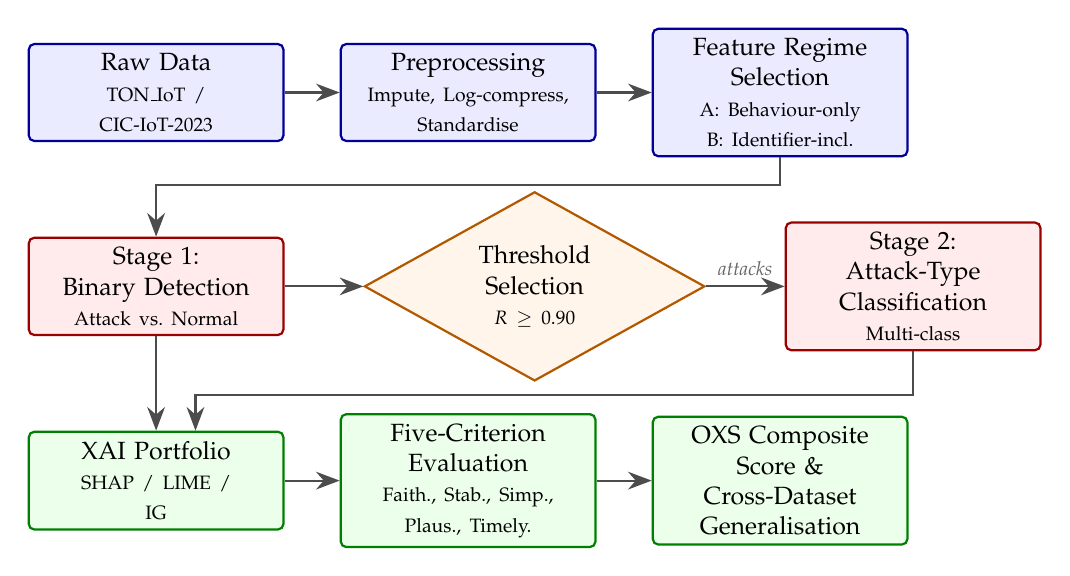
\begin{tikzpicture}[
    node distance=1.2cm and 0.7cm,
    >={Stealth[length=3mm]},
    block/.style={rectangle, draw=blue!60!black, fill=blue!8, text width=3.0cm, minimum height=1.2cm, align=center, font=\small, rounded corners=2pt, line width=0.8pt},
    stage/.style={rectangle, draw=red!60!black, fill=red!8, text width=3.0cm, minimum height=1.2cm, align=center, font=\small, rounded corners=2pt, line width=0.8pt},
    decision/.style={diamond, draw=orange!70!black, fill=orange!8, text width=1.8cm, minimum height=1.0cm, align=center, font=\small, aspect=1.8, line width=0.8pt},
    output/.style={rectangle, draw=green!50!black, fill=green!8, text width=3.0cm, minimum height=1.2cm, align=center, font=\small, rounded corners=2pt, line width=0.8pt},
    arrow/.style={->, line width=0.8pt, draw=black!70},
    lbl/.style={font=\scriptsize\itshape, text=black!60}
]

% Row 1: Data pipeline
\node[block] (raw) {Raw Data\\{\scriptsize TON\_IoT /}\\{\scriptsize CIC-IoT-2023}};
\node[block, right=of raw] (preproc) {Preprocessing\\{\scriptsize Impute, Log-compress,}\\{\scriptsize Standardise}};
\node[block, right=of preproc] (regime) {Feature Regime\\Selection\\{\scriptsize A: Behaviour-only}\\{\scriptsize B: Identifier-incl.}};

% Row 2: Detection pipeline
\node[stage, below=of raw] (stage1) {Stage~1:\\Binary Detection\\{\scriptsize Attack vs.\ Normal}};
\node[decision, right=1.0cm of stage1] (thresh) {Threshold\\Selection\\{\scriptsize $R \geq 0.90$}};
\node[stage, right=1.0cm of thresh] (stage2) {Stage~2:\\Attack-Type\\Classification\\{\scriptsize Multi-class}};

% Row 3: Explanation and evaluation
\node[output, below=of stage1] (xai) {XAI Portfolio\\{\scriptsize SHAP / LIME /}\\{\scriptsize IG}};
\node[output, right=of xai] (eval) {Five-Criterion\\Evaluation\\{\scriptsize Faith., Stab., Simp.,}\\{\scriptsize Plaus., Timely.}};
\node[output, right=of eval] (oxs) {OXS Composite\\Score \&\\Cross-Dataset\\Generalisation};

% === Arrows ===

% Row 1: horizontal
\draw[arrow] (raw.east) -- (preproc.west);
\draw[arrow] (preproc.east) -- (regime.west);

% Row 1 to Row 2: vertical down from regime, then horizontal to stage1
\draw[arrow] (regime.south) -- ++(0,-0.35) -| (stage1.north);

% Row 2: horizontal
\draw[arrow] (stage1.east) -- (thresh.west);
\draw[arrow] (thresh.east) -- node[above, lbl] {attacks} (stage2.west);

% Row 2 to Row 3: stage1 down to xai
\draw[arrow] (stage1.south) -- (xai.north);
% Stage 2 down then left to XAI (route outside, connects cleanly)
\draw[arrow] (stage2.south) -- ++(0,-0.55) -| ([xshift=0.5cm]xai.north);

% Row 3: horizontal
\draw[arrow] (xai.east) -- (eval.west);
\draw[arrow] (eval.east) -- (oxs.west);

\end{tikzpicture}
\caption{HYDRA pipeline architecture. Raw data flows through preprocessing and feature regime selection into the two-stage detection pipeline. Both stages feed into the XAI portfolio, which is assessed against five criteria and aggregated into the OXS composite score. Cross-dataset generalisation is evaluated at the detection level.}
\label{fig:pipeline}
\end{figure}

\section{Datasets and Preprocessing}
\label{sec:datasets}

\subsection{TON\_IoT}
\label{sec:toniot-meth}

TON\_IoT \cite{moustafa2021} comprises approximately 211,000 bidirectional network flow records extracted using the Zeek network monitor. Each row is characterised by connection metadata (source/destination IP, port, protocol), volumetric statistics (bytes and packets in each direction), and the flow duration. The dataset contains nine attack types (DoS, DDoS, scanning, ransomware, backdoor, injection, XSS, password, and MitM) alongside normal traffic, with 76\% attack prevalence. Source IP addresses enable group-disjoint splitting. The raw dataset contains 9.7\% exact duplicate rows (20,569 of 211,043); a deduplication step removes these prior to splitting, yielding 190,474 unique rows for all experiments.

\begin{figure}[htbp]
\centering
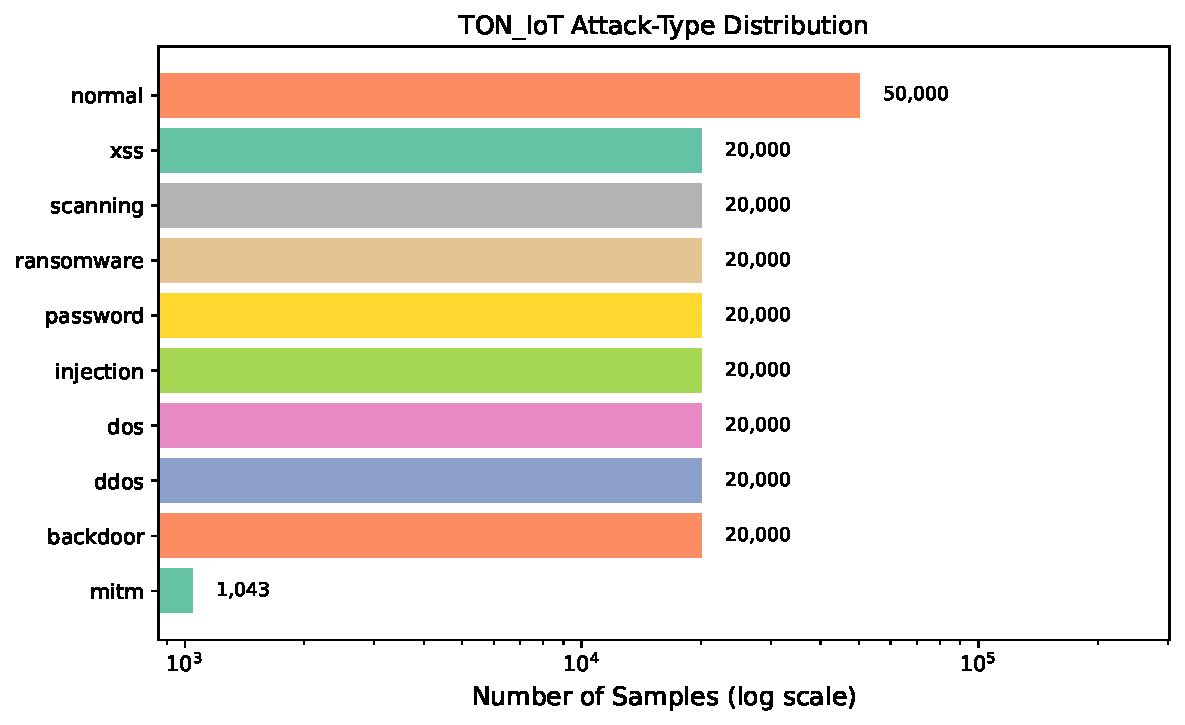
\includegraphics[width=0.8\textwidth]{figures/class_distribution_toniot.pdf}
\caption{Class distribution of TON\_IoT dataset (log scale).}
\label{fig:class-dist}
\end{figure}

\subsection{CIC-IoT-2023}
\label{sec:ciciot-meth}

CIC-IoT-2023 \cite{cic2023} comprises approximately 3.18 million flow records after deduplication. The raw dataset contained 44\% duplicate rows; a preprocessing step computes SHA-256 hashes and removes exact duplicates to prevent train--test leakage. After deduplication, the dataset contains 34 attack types with 97.7\% attack prevalence. Features include protocol flags (TCP, UDP, ICMP), aggregate packet statistics, and statistical summaries. It lacks IP and timestamp columns, constraining splitting strategies and precluding GNN evaluation.

\subsection{Preprocessing Pipeline}
\label{sec:preprocess}

The preprocessing pipeline is fitted exclusively on the training partition to prevent information leakage. It applies three sequential transformations:

\begin{enumerate}
  \item \textbf{Median imputation}: missing numeric values are replaced with the training-set median. Categorical missing values are imputed with the most frequent training-set value.
  \item \textbf{Log-compression}: a $\log(1 + x)$ transformation is applied to all non-negative numeric features after clipping negative values to zero, compressing the right-skewed distributions characteristic of network flow volumes.
  \item \textbf{Standardisation}: each numeric feature is centred to zero mean and scaled to unit variance using training-set statistics. While tree-based models are scale-invariant, this step benefits logistic regression and the CNN-LSTM.
\end{enumerate}

Categorical features undergo most-frequent imputation followed by one-hot encoding with unknown-category handling.

\section{Feature Regimes}
\label{sec:regimes}

\textbf{Regime A (Behaviour-only)} retains only traffic-behavioural features: flow duration, byte counts (source and destination), packet counts, protocol metadata, and connection state indicators. It explicitly excludes IP addresses, port numbers, service labels, and high-cardinality string fields. By removing identifiers, Regime~A forces models to learn from traffic patterns alone, producing explanations that reference only operationally meaningful features.

\textbf{Regime B (Identifier-inclusive)} augments Regime~A with network identifiers: source and destination IP addresses, port numbers, and service labels. This permits models to exploit identity-based shortcuts, for example memorising that a specific source IP is always associated with attacks.

The distinction serves a dual purpose. For detection, it quantifies the performance gap attributable to identifier leakage. For explainability, it tests whether Regime~B models produce explanations dominated by identifier features that offer no actionable insight (Appendix~\ref{app:features}).

\section{Data Splitting Strategies}
\label{sec:splitting}

HYDRA implements three data splitting strategies, each producing disjoint train/validation/test partitions.

\textbf{Stratified split} uses scikit-learn's \texttt{StratifiedShuffleSplit} to preserve class distribution across all partitions. It is the primary strategy because it guarantees sufficient positive and negative samples in each split.

\textbf{Host split} groups flows by source IP and assigns entire hosts to a single partition, ensuring no IP appears in more than one split. This prevents models from memorising host-specific patterns and simulates deployment against unseen devices. Applicable only to TON\_IoT.

\textbf{Host-type-aware split} extends host splitting with a greedy pinning algorithm that guarantees all attack types appear in training by pinning the host with the most samples of each type (rarest first).

All strategies enforce non-empty partitions, no NaN labels, and class-presence warnings. Stratified splitting is primary; host-disjoint splits serve as supplementary deployment-realistic analyses. Temporal splitting is supported by the pipeline implementation but is not reported here because TON\_IoT lacks a timestamp column and CIC-IoT-2023 was released without per-flow timestamps.

\section{Model Selection and Architecture}
\label{sec:models}

Two non-learned baselines establish lower bounds. The \textbf{majority-class baseline} assigns every flow a score equal to the training-set attack prevalence. The \textbf{threshold baseline} computes a heuristic anomaly score as $\log(1 + \text{duration}) + \log(1 + \text{total\_bytes}) + \log(1 + \text{total\_packets})$, capturing the intuition that anomalous flows exhibit unusual volume or duration.

\textbf{Logistic Regression} serves as the reference explainable model whose linear decision boundary yields deterministic attributions via SHAP LinearExplainer.

\textbf{Random Forest} uses 100 estimators, maximum depth 15, and balanced class weights. \textbf{XGBoost} uses 400 boosting rounds, learning rate 0.05, maximum depth 8, and \texttt{scale\_pos\_weight} for class imbalance. \textbf{LightGBM} uses 400 estimators, learning rate 0.05, and \texttt{num\_leaves=64}. All hyperparameters follow literature defaults; sensitivity analysis is future work (Section~\ref{sec:limitations}).

\textbf{CNN-LSTM}: Two Conv1d layers capture local feature interactions, followed by an LSTM layer for sequential structure, global average pooling, and a fully connected head with dropout 0.3. Training uses Adam with cosine annealing over 50 epochs and early stopping (patience 10).

\textbf{GNN (GraphSAGE)}: Models traffic as a communication graph (nodes = IP addresses, edges = flows). Two SAGEConv layers with max-aggregation learn node embeddings; an edge MLP concatenates source/destination embeddings with edge features for classification. Applicable only to datasets with IP columns (TON\_IoT).

\section{Two-Stage Classification Pipeline}
\label{sec:two-stage}

\textbf{Stage 1 (Binary Detection)} trains a classifier on all flows to distinguish attacks from normal traffic. The model outputs a continuous score representing attack probability. An operating threshold is selected on the validation set to maximise precision subject to achieving at least 90\% recall.

\textbf{Stage 2 (Multiclass Type Classification)} trains a separate classifier exclusively on training flows labelled as attacks. At inference, flows that Stage~1 classifies as attacks are passed to Stage~2 for type prediction. Flows classified as normal by Stage~1 are assigned the normal type label without consulting Stage~2.

Evaluation reports both \textbf{end-to-end accuracy} (including Stage~1 misclassifications) and \textbf{detected-only accuracy} (Stage~2 performance on correctly flagged attacks), alongside macro-F1 and weighted-F1.

\section{Evaluation Metrics}
\label{sec:metrics}

\textbf{PR-AUC (Average Precision)} is the primary ranking metric, chosen for its robustness to class imbalance. Under severe imbalance, ROC-AUC can be misleadingly high because the false positive rate denominator is dominated by the majority class. A sanity check verifies that a constant score equal to the prevalence yields PR-AUC equal to the prevalence.

\textbf{ROC-AUC} is reported alongside PR-AUC. For cross-dataset experiments where CIC-IoT-2023's 97.7\% prevalence inflates PR-AUC, ROC-AUC provides the more informative comparison.

The operating threshold is selected on the validation set to maximise precision at recall $\geq 0.90$, yielding test-set precision, FPR, and coverage. Stage~2 uses \textbf{macro-F1} (equal weight to rare types) and \textbf{weighted-F1}.

The \textbf{DeLong paired AUC test} \cite{delong1988} assesses statistical significance for all model pairs on the same test set. Each experiment uses three random seeds (21, 42, 84), with results reported as mean $\pm$ standard deviation. Two automated leakage audits (PR-AUC sanity check and SHA-256 row-hash duplicate detection across partitions) guard against data leakage.

\section{Explainability Methods}
\label{sec:xai-methods}

For tree-based models (Random Forest, XGBoost, LightGBM, sklearn GBDT), SHAP TreeExplainer \cite{lundberg2020} computes exact Shapley values by exploiting the tree structure. Each feature receives a signed attribution indicating its contribution toward the attack or normal class. For multiclass models, SHAP values are computed per class.

For logistic regression, LinearExplainer computes analytically exact Shapley values using the model's coefficient vector and an independent masker, providing a deterministic, computationally inexpensive attribution baseline.

LIME \cite{ribeiro2016} provides model-agnostic local explanations by fitting a sparse linear model to each instance's neighbourhood. For each of 50 sampled validation instances, 2,000 perturbations are generated, enabling direct cross-model comparison.

For the CNN-LSTM and the GNN, Integrated Gradients \cite{sundararajan2017} computes the path integral from a zero baseline to the actual input using 50 interpolation steps (Equation~\ref{eq:ig}). The zero baseline represents ``no network traffic.'' IG is preferred over GradientExplainer because MaxPool1d introduces non-differentiable points. For the GNN, IG is applied to edge features; full quantitative XAI evaluation of GNN attributions under the five-criterion protocol is identified as future work.

\begin{equation}
\label{eq:ig}
\text{IG}_i(x, x') = (x_i - x'_i) \times \int_0^1 \frac{\partial f(x' + \alpha(x - x'))}{\partial x_i} \, d\alpha
\end{equation}

\section{Five-Criterion XAI Evaluation Protocol}
\label{sec:five-criterion}

\subsection{Faithfulness}
\label{sec:faithfulness}

Faithfulness measures whether the features highlighted by an explanation actually drive the model's prediction. Two complementary tests are used with $k = 5$. \textbf{Comprehensiveness}: replace the top-$k$ features with the training-set median (a neutral baseline) and measure the drop in model confidence; a large drop means those features genuinely mattered (higher = more faithful). \textbf{Sufficiency}: keep only the top-$k$ features (replacing all others with medians) and measure how much confidence is retained; if the top features are sufficient, confidence stays high (lower difference = more faithful).
\begin{equation}
\text{Comp}(x, S_k) = f(x) - f(x_{\setminus S_k}), \quad \text{Suff}(x, S_k) = f(x) - f(x_{S_k})
\end{equation}

\subsection{Stability}
\label{sec:stability}

Stability measures whether an explanation changes when the input or model is slightly perturbed. \textbf{S1 (Seed stability)}: retrain the model with $S = 5$ different random seeds and compare the resulting explanations using Spearman $\rho$ across all $\binom{5}{2} = 10$ seed pairs. \textbf{S2 (Noise stability)}: add small Gaussian noise ($\sigma = 0.01 \times \text{std}(X_j)$) to the input over $R = 20$ draws and compute Spearman $\rho$ between the original and noisy feature rankings (higher $\rho$ = more stable). The present evaluation reports S2 only; S1 is identified as priority future work (Section~\ref{sec:limitations}).

\subsection{Simplicity}
\label{sec:simplicity}

Simplicity measures whether an explanation is concise enough for an analyst to act on. \textbf{$k_{90}$}: the minimum number of features needed to account for 90\% of the total attribution mass, normalised by total features (lower = simpler). \textbf{Gini coefficient}: measures how concentrated the attribution distribution is (higher = fewer features dominate, simpler explanation).

\subsection{Plausibility}
\label{sec:plausibility}

Plausibility measures whether the features highlighted by an explanation match what a domain expert would expect for a given attack type. RMA@$k$ compares the top-$k$ attributed features against reference sets compiled from attack descriptions in the TON\_IoT documentation \cite{moustafa2021} and IDS feature importance studies \cite{shtayat2023} (higher = better alignment; Table~\ref{tab:reference} in Appendix~\ref{app:formulae}):
\begin{equation}
\text{RMA@}k = \frac{|\text{top-}k \text{ features} \cap \text{reference set}|}{k}
\end{equation}

\subsection{Timeliness}
\label{sec:timeliness}

Timeliness measures whether explanations can be generated fast enough for real-time use. It is reported as wall-clock milliseconds per sample, averaged over 200 test instances (three repetitions).

\subsection{OXS Composite Score}
\label{sec:oxs}

Each criterion is normalised to $[0, 1]$: faithfulness uses $\max(0, \text{Comp})$ clipped to 1; stability and plausibility are already bounded correlations and proportions; simplicity averages $(1 - k_{90})$ and Gini; timeliness is mapped via $1 / (1 + t / 1000)$, where 1000\,ms represents a practical upper bound for interactive SOC triage. The five normalised scores are aggregated with equal weights:
\begin{multline}
\text{OXS} = 0.2 \times \text{Faithfulness} + 0.2 \times \text{Stability} + 0.2 \times \text{Simplicity} \\
 + \; 0.2 \times \text{Plausibility} + 0.2 \times \text{Timeliness}
\end{multline}

\section{Cross-Dataset Generalisation}
\label{sec:cross-dataset}

\subsection{Canonical Feature Alignment}
\label{sec:alignment}

Six canonical features are mapped across datasets (Table~\ref{tab:canonical}).

\begin{table}[H]
\centering
\caption{Canonical feature alignment for cross-dataset generalisation.}
\label{tab:canonical}
\begin{adjustbox}{max width=\textwidth}
\begin{tabular}{lll}
\toprule
\textbf{Canonical Feature} & \textbf{TON\_IoT Derivation} & \textbf{CIC-IoT-2023 Column} \\
\midrule
\texttt{f\_total\_pkts} & \texttt{src\_pkts + dst\_pkts} & \texttt{number} \\
\texttt{f\_total\_bytes} & \texttt{src\_bytes + dst\_bytes} & \texttt{tot\_size} \\
\texttt{f\_duration} & \texttt{duration} & \texttt{iat} \\
\texttt{f\_is\_tcp} & \texttt{(proto == `tcp').astype(int)} & \texttt{tcp} \\
\texttt{f\_is\_udp} & \texttt{(proto == `udp').astype(int)} & \texttt{udp} \\
\texttt{f\_is\_icmp} & \texttt{(proto == `icmp').astype(int)} & \texttt{icmp} \\
\bottomrule
\end{tabular}
\end{adjustbox}
\end{table}

\subsection{Experimental Protocol}
\label{sec:cross-protocol}

For each direction, the source dataset is aligned, split, and preprocessed; the target is transformed using source-fitted preprocessing. Binary classifiers are trained on source and evaluated on both source-test and the full target. ROC-AUC is the primary metric due to CIC-IoT-2023's prevalence inflation of PR-AUC.

\section{Leakage Interaction Analysis}
\label{sec:leakage-interaction}

Each model is trained twice under identical conditions: once under Regime~A (behaviour-only) and once under Regime~B (identifier-inclusive), producing $n = 4$ paired observations (one per tabular model). For each pair, the difference in per-attack-type plausibility (RMA@5) and detection metrics is computed. Cohen's $d$ on these paired differences quantifies the effect size of identifier inclusion on explanation quality, testing whether the observed plausibility degradation is systematic rather than model-specific.

\section{Reproducibility and Implementation}
\label{sec:implementation}

HYDRA is implemented in Python 3.11. Every run records Git commit hash, dataset fingerprint (SHA-256), package versions, and full configuration. A test suite of 91 automated tests covers splitting invariants, metric computation, baselines, model building, and XAI functions. Continuous integration runs on every push. The project was conducted over 8 months (October 2025 to May 2026).

\section{Ethical Considerations}
\label{sec:ethics}

Both datasets (TON\_IoT and CIC-IoT-2023) are publicly available, pre-anonymised benchmarks released for research use by their respective institutions. No personal data was processed, no operational IDS was deployed, and no real network traffic was intercepted. The project was conducted in accordance with the University of Bath's ethical review framework; formal ethics approval was not required as the work involves only publicly available, anonymised datasets with no human participants.

% ============================================================
% CHAPTER 4: RESULTS
% ============================================================
\chapter{Results}
\label{ch:results}

This chapter presents the experimental results obtained from the HYDRA framework across four evaluation dimensions: detection performance (Sections~\ref{sec:binary-results}--\ref{sec:multiclass-results}), deep learning models (Section~\ref{sec:cnnlstm-results}), explainability quality (Sections~\ref{sec:xai-results}--\ref{sec:oxs-results}), and cross-dataset generalisation (Section~\ref{sec:cross-results}). Section~\ref{sec:leakage-results} examines the interaction between identifier leakage and explanation quality. All experiments follow the protocols described in Chapter~\ref{ch:methodology}.

\section{Experimental Setup}
\label{sec:setup}

All within-dataset experiments use the TON\_IoT dataset \cite{alsaedi2020}, comprising 190,474 network flow records after deduplication (76\% attack prevalence). A stratified train/validation/test split is applied with three random seeds (21, 42, 84) to provide variance estimates. Two feature regimes are evaluated: \textbf{behaviour-only} (dropping source/destination IP addresses, ports, and service identifiers before training) and \textbf{identifier-inclusive} (retaining all features). Four tabular model families are compared (Logistic Regression (LogReg), Random Forest, XGBoost, and LightGBM) alongside CNN-LSTM and GNN deep learning models. The two-stage pipeline performs binary detection (benign vs.\ attack) in Stage~1 and nine-class attack-type classification in Stage~2.

\section{Binary Detection Performance}
\label{sec:binary-results}

Table~\ref{tab:binary} reports three-seed-averaged binary detection results.

\begin{table}[H]
\centering
\caption{Binary detection performance on TON\_IoT (3-seed average $\pm$ standard deviation, deduplicated, stratified split).}
\label{tab:binary}
\begin{adjustbox}{max width=\textwidth}
\begin{tabular}{llccc}
\toprule
\textbf{Model} & \textbf{Regime} & \textbf{PR-AUC} & \textbf{ROC-AUC} & \textbf{Binary F1} \\
\midrule
XGBoost & Behaviour-only & $1.000 \pm 0.000$ & $0.9999 \pm 0.000$ & $0.9999 \pm 0.000$ \\
LightGBM & Behaviour-only & $1.000 \pm 0.000$ & $0.9999 \pm 0.000$ & $0.9999 \pm 0.000$ \\
Random Forest & Behaviour-only & $0.9999 \pm 0.000$ & $0.9997 \pm 0.000$ & $0.9998 \pm 0.000$ \\
LogReg & Behaviour-only & $0.9984 \pm 0.000$ & $0.9959 \pm 0.001$ & $0.9956 \pm 0.001$ \\
\midrule
XGBoost & Identifier-incl & $1.000 \pm 0.000$ & $1.000 \pm 0.000$ & $1.000 \pm 0.000$ \\
LightGBM & Identifier-incl & $1.000 \pm 0.000$ & $1.000 \pm 0.000$ & $1.000 \pm 0.000$ \\
Random Forest & Identifier-incl & $1.000 \pm 0.000$ & $1.000 \pm 0.000$ & $1.000 \pm 0.000$ \\
LogReg & Identifier-incl & $1.000 \pm 0.000$ & $0.9999 \pm 0.000$ & $0.9999 \pm 0.000$ \\
\bottomrule
\end{tabular}
\end{adjustbox}
\end{table}

The binary detection task on TON\_IoT is effectively solved: all four tabular models achieve PR-AUC $\geq 0.998$ and ROC-AUC $\geq 0.996$ under the behaviour-only regime. Identifier-inclusive results are marginally higher (PR-AUC $= 1.000$ for all models), indicating that identifiers provide a small additional shortcut but are not required for near-perfect binary detection.

LogReg achieving PR-AUC $= 0.998$ under the behaviour-only regime confirms that the binary task is nearly linearly separable in the behavioural feature space, consistent with \cite{alsaedi2020} and \cite{moustafa2021}. DeLong paired AUC tests confirm that inter-model differences are not statistically significant at the binary level ($p > 0.05$ for all pairs), reinforcing the conclusion that binary detection does not discriminate between models on this dataset. The multiclass task and XAI evaluation provide greater differentiation.

\subsection{Split Strategy Impact on Detection Performance}
\label{sec:split-impact}

Table~\ref{tab:split-impact} compares stratified versus host-disjoint splitting on the deduplicated dataset (190,474 rows).

\begin{table}[H]
\centering
\caption{Impact of splitting strategy on detection performance (behaviour-only, deduplicated TON\_IoT).}
\label{tab:split-impact}
\begin{adjustbox}{max width=\textwidth}
\begin{tabular}{llcc}
\toprule
\textbf{Model} & \textbf{Split} & \textbf{ROC-AUC} & \textbf{F1} \\
\midrule
XGBoost & Stratified & 0.9999 & 0.9999 \\
XGBoost & Host-disjoint & 0.854 & 0.932 \\
CNN-LSTM & Stratified & 0.9974 & 0.928 \\
CNN-LSTM & Host-disjoint & 0.834 & 0.873 \\
LogReg & Host-disjoint & 0.538 & 0.923 \\
\bottomrule
\end{tabular}
\end{adjustbox}
\end{table}

\textbf{The stratified split inflates XGBoost's ROC-AUC from 0.854 to 0.9999}, a 14.6 percentage point gap, even after deduplication and identifier removal. This occurs because stratified splitting allows flows from the same source host to appear in both partitions, and flows from the same host share near-identical behavioural signatures.

Feature importance under the host split confirms this: \texttt{conn\_state\_S0} accounts for 54\% of feature importance, followed by \texttt{proto\_tcp} (20\%) and \texttt{conn\_state\_SF} (10\%). Certain connection states (\texttt{REJ}: 100\% attack prevalence, \texttt{S1}: 99.9\%) are near-deterministic indicators.

The host-split ROC-AUC of 0.854 represents a more realistic deployment estimate. LogReg's host-split ROC-AUC of 0.538 (barely above random) demonstrates that linear separability does not transfer to unseen hosts. Stratified results remain valuable for XAI comparison but should not be interpreted as deployment-realistic.

\subsection{Host-Disjoint Multiclass Attack-Type Classification}
\label{sec:host-multiclass}

Table~\ref{tab:host-multiclass} presents multiclass results under host-disjoint splitting.

\begin{table}[H]
\centering
\caption{Host-disjoint multiclass attack-type classification (behaviour-only, 20,000-row balanced test subsample).}
\label{tab:host-multiclass}
\resizebox{\textwidth}{!}{%
\begin{tabular}{lcccccccccc}
\toprule
\textbf{Model} & \textbf{Macro-F1} & \textbf{Wtd-F1} & \textbf{Back.} & \textbf{DDoS} & \textbf{DoS} & \textbf{Inj.} & \textbf{MitM} & \textbf{Pass.} & \textbf{Ransom.} & \textbf{Scan.} \\
\midrule
Random Forest & \textbf{0.742} & 0.952 & 0.907 & 0.955 & 0.060 & 0.982 & 0.104 & 0.988 & 0.994 & 0.944 \\
XGBoost & 0.682 & 0.957 & 0.287 & 0.955 & 0.080 & 0.979 & 0.191 & 0.984 & 0.992 & 0.987 \\
LightGBM & 0.732 & 0.953 & 0.926 & 0.948 & 0.074 & 0.985 & 0.000 & 0.984 & 0.994 & 0.949 \\
LogReg & 0.571 & 0.866 & 0.053 & 0.916 & 0.054 & 0.954 & 0.000 & 0.823 & 0.947 & 0.820 \\
\bottomrule
\end{tabular}%
}
\end{table}

The results reveal four findings invisible under stratified splitting. First, \textbf{multiclass macro-F1 drops from 0.952 to 0.742 (host-disjoint) for the best model}, a 21 percentage point decrease demonstrating that stratified results reflect host-level memorisation rather than generalisable attack-type discrimination.

Second, \textbf{DoS is the hardest attack type} (maximum F1 = 0.080), systematically confused with DDoS due to similar volumetric signatures at the flow level; distinguishing them requires session-level or source-count features lost in per-flow aggregation. MitM remains unstable (maximum F1 = 0.191) with only 4 test samples.

Third, \textbf{six of eight attack types achieve F1 $> 0.82$ for the best model}: Ransomware (0.994), Password (0.988), Injection (0.982), DDoS (0.955), Scanning (0.944), and Backdoor (0.907), indicating the challenge is concentrated on DoS and MitM. Fourth, \textbf{the model ranking changes}: Random Forest (0.742) outperforms XGBoost (0.682), reversing the stratified ranking.

\section{Multi-Class Attack-Type Classification}
\label{sec:multiclass-results}

Table~\ref{tab:multiclass} presents stratified multiclass results.

\begin{table}[H]
\centering
\caption{Multiclass attack-type classification on TON\_IoT (3-seed average $\pm$ standard deviation, deduplicated).}
\label{tab:multiclass}
\begin{adjustbox}{max width=\textwidth}
\begin{tabular}{llcc}
\toprule
\textbf{Model} & \textbf{Regime} & \textbf{Macro-F1} & \textbf{Weighted-F1} \\
\midrule
XGBoost & Behaviour-only & $0.952 \pm 0.002$ & $0.979 \pm 0.001$ \\
LightGBM & Behaviour-only & $0.955 \pm 0.004$ & $0.984 \pm 0.002$ \\
Random Forest & Behaviour-only & $0.930 \pm 0.029$ & $0.981 \pm 0.002$ \\
LogReg & Behaviour-only & $0.813 \pm 0.019$ & $0.901 \pm 0.002$ \\
\midrule
XGBoost & Identifier-incl & $0.986 \pm 0.001$ & $0.995 \pm 0.001$ \\
LightGBM & Identifier-incl & $0.987 \pm 0.001$ & $0.995 \pm 0.000$ \\
Random Forest & Identifier-incl & $0.957 \pm 0.001$ & $0.987 \pm 0.001$ \\
LogReg & Identifier-incl & $0.966 \pm 0.002$ & $0.984 \pm 0.001$ \\
\bottomrule
\end{tabular}
\end{adjustbox}
\end{table}

LightGBM achieves the highest behaviour-only macro-F1 ($0.955 \pm 0.004$), followed closely by XGBoost ($0.952 \pm 0.002$) and Random Forest ($0.930 \pm 0.029$). LogReg's lower macro-F1 ($0.813 \pm 0.019$) reflects difficulty distinguishing attack types with similar volumetric profiles using a linear boundary.

\textbf{Identifiers substantially improve multiclass performance}: LogReg macro-F1 rises from 0.813 to 0.966 ($+0.153$), confirming that IP-level patterns provide strong linear signal for type discrimination. XGBoost gains a smaller but consistent $+0.034$, while Random Forest gains $+0.027$.

\subsection{Within-Dataset Multiclass on CIC-IoT-2023}
\label{sec:cic-multiclass}

To validate the dual-task pipeline on a second dataset, the same four tabular models were trained on CIC-IoT-2023 (34 attack types). Because CIC-IoT-2023 lacks IP, port, and service columns, the two feature regimes are equivalent here; results are reported once.

\begin{table}[H]
\centering
\caption{Multiclass attack-type classification on CIC-IoT-2023 (3-seed mean $\pm$ std, 500{,}000-row stratified subsample of the deduplicated 3.18M-row dataset, 34 attack types). The behaviour-only and identifier-inclusive regimes are equivalent because CIC-IoT-2023 contains no IP, port, or service columns.}
\label{tab:multiclass-cic}
\begin{adjustbox}{max width=\textwidth}
\begin{tabular}{lcc}
\toprule
\textbf{Model} & \textbf{Macro-F1} & \textbf{Weighted-F1} \\
\midrule
Random Forest & $\mathbf{0.887 \pm 0.047}$ & $0.998 \pm 0.000$ \\
XGBoost & $0.810 \pm 0.011$ & $0.998 \pm 0.000$ \\
LogReg & $0.644 \pm 0.034$ & $0.827 \pm 0.001$ \\
LightGBM & $0.152 \pm 0.045$ & $0.335 \pm 0.120$ \\
\bottomrule
\end{tabular}
\end{adjustbox}
\end{table}

\textbf{Random Forest achieves the highest macro-F1 (0.887)}, ahead of XGBoost (0.810) and LogReg (0.644); reversing the TON\_IoT ranking. Bagging's variance reduction is more robust than gradient boosting under CIC-IoT-2023's 34-class extreme class imbalance, where rare attack subtypes are easily underfit by boosted models. \textbf{LightGBM's default configuration failed} (macro-F1 $= 0.152$); the default \texttt{min\_data\_in\_leaf} is too high for the rare classes, causing premature termination. Tuning is future work.

CNN-LSTM was not re-evaluated on CIC-IoT-2023: at 3.18M rows the dataset is $\sim$17$\times$ larger than TON\_IoT and a single training seed would require an estimated 40+ hours.

Table~\ref{tab:perclass-f1} reports the end-to-end two-stage pipeline accuracy for XGBoost, demonstrating that Stage~2 achieves 0.979 accuracy on correctly detected attacks.

\begin{table}[H]
\centering
\caption{Two-stage type classification accuracy for XGBoost under the behaviour-only regime (seed 42, deduplicated).}
\label{tab:perclass-f1}
\begin{adjustbox}{max width=\textwidth}
\begin{tabular}{lc}
\toprule
\textbf{Metric} & \textbf{Value} \\
\midrule
End-to-end type accuracy & 0.960 \\
Attack-only accuracy & 0.949 \\
Attack accuracy (detected only) & 0.979 \\
Macro-F1 & 0.950 \\
Weighted-F1 & 0.979 \\
\bottomrule
\end{tabular}
\end{adjustbox}
\end{table}

\section{Deep Learning Results: CNN-LSTM and GNN}
\label{sec:cnnlstm-results}

An earlier CNN-LSTM version suffered convergence failure, resolved through five architectural fixes: explicit LSTM hidden-state initialisation, Kaiming weight initialisation, unconditional \texttt{pos\_weight}, zero-padding for odd-length sequences, and gradient clipping.

\begin{figure}[htbp]
\centering
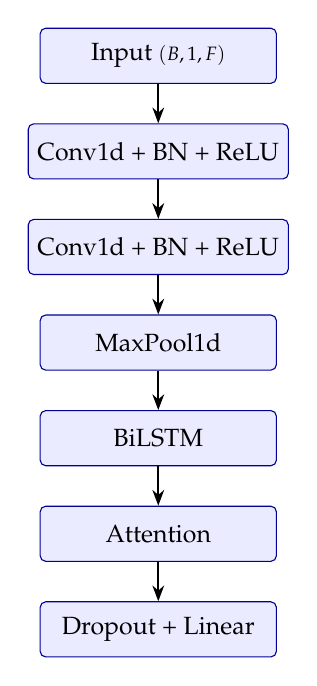
\begin{tikzpicture}[
    node distance=0.5cm,
    layer/.style={rectangle, draw=blue!60!black, fill=blue!8, minimum width=3cm, minimum height=0.7cm, align=center, font=\small, rounded corners=2pt},
    arrow/.style={->, >=Stealth, line width=0.6pt}
]
\node[layer] (input) {Input {\scriptsize $(B, 1, F)$}};
\node[layer, below=of input] (conv1) {Conv1d + BN + ReLU};
\node[layer, below=of conv1] (conv2) {Conv1d + BN + ReLU};
\node[layer, below=of conv2] (pool) {MaxPool1d};
\node[layer, below=of pool] (lstm) {BiLSTM};
\node[layer, below=of lstm] (attn) {Attention};
\node[layer, below=of attn] (fc) {Dropout + Linear};

\draw[arrow] (input) -- (conv1);
\draw[arrow] (conv1) -- (conv2);
\draw[arrow] (conv2) -- (pool);
\draw[arrow] (pool) -- (lstm);
\draw[arrow] (lstm) -- (attn);
\draw[arrow] (attn) -- (fc);
\end{tikzpicture}
\caption{CNN-LSTM architecture with attention mechanism.}
\label{fig:cnn-lstm-arch}
\end{figure}

\subsection{CNN-LSTM Detection Performance}
\label{sec:cnnlstm-detection}

\begin{table}[H]
\centering
\caption{CNN-LSTM detection results (behaviour-only regime, deduplicated, 3-seed average).}
\label{tab:cnnlstm}
\begin{adjustbox}{max width=\textwidth}
\begin{tabular}{lc}
\toprule
\textbf{Metric} & \textbf{Value} \\
\midrule
Binary PR-AUC & $0.9992 \pm 0.0007$ \\
Binary ROC-AUC & $0.9974 \pm 0.0022$ \\
Multiclass Macro-F1 & $0.928 \pm 0.000$ \\
Training time & $\sim$150 min per seed \\
\bottomrule
\end{tabular}
\end{adjustbox}
\end{table}

Under host-disjoint evaluation, ROC-AUC drops from 0.9974 to 0.7614 (Table~\ref{tab:cnnlstm-host}), confirming stratified inflation even without identifiers.

\begin{table}[H]
\centering
\caption{CNN-LSTM binary detection under host-disjoint split (behaviour-only, deduplicated).}
\label{tab:cnnlstm-host}
\begin{adjustbox}{max width=\textwidth}
\begin{tabular}{lcc}
\toprule
\textbf{Metric} & \textbf{Stratified} & \textbf{Host Split} \\
\midrule
Binary PR-AUC & 0.9992 & 0.9531 \\
Binary ROC-AUC & 0.9974 & 0.7614 \\
Binary F1 & 0.928 & 0.7735 \\
\bottomrule
\end{tabular}
\end{adjustbox}
\end{table}

\subsection{CNN-LSTM XAI Evaluation}
\label{sec:cnnlstm-xai}

\begin{table}[H]
\centering
\caption{CNN-LSTM XAI five-criterion evaluation via Integrated Gradients.}
\label{tab:cnnlstm-xai}
\begin{adjustbox}{max width=\textwidth}
\begin{tabular}{lc}
\toprule
\textbf{Criterion} & \textbf{Value} \\
\midrule
Comprehensiveness & $-0.052$ \\
Sufficiency & $1.000$ \\
S2 (noise stability) & 0.713 \\
$k_{90}$ & 0.137 \\
Gini coefficient & 0.858 \\
RMA@5 (mean) & 0.600 \\
IG timing & 2.46 ms/sample \\
\bottomrule
\end{tabular}
\end{adjustbox}
\end{table}

The CNN-LSTM's $k_{90}$ (0.137) matches XGBoost's tabular value (0.131), and its plausibility (RMA@5 $= 0.60$) sits between LightGBM and XGBoost. Top IG features are volumetric (\texttt{src\_bytes}, \texttt{dst\_bytes}, \texttt{src\_pkts}).

\subsection{GNN Detection Performance}
\label{sec:gnn-results}

\begin{table}[H]
\centering
\caption{GNN (GraphSAGE) detection results on TON\_IoT (deduplicated, stratified split, seed 42).}
\label{tab:gnn}
\begin{adjustbox}{max width=\textwidth}
\begin{tabular}{lc}
\toprule
\textbf{Metric} & \textbf{Value} \\
\midrule
Binary PR-AUC & 0.9993 \\
Binary ROC-AUC & 0.9988 \\
Binary F1 & 0.9952 \\
Training time & $\sim$3 min (binary) + $\sim$1.7 h (XAI) \\
\bottomrule
\end{tabular}
\end{adjustbox}
\end{table}

The GNN achieves binary detection close to tree ensembles, demonstrating graph structure is effective for IDS. It is TON\_IoT-only (requires IP columns). Multiclass GraphSAGE adaptation is future work; the binary edge classifier does not natively predict attack type.

\subsection{Cross-Architecture Comparison}
\label{sec:arch-comparison}

\begin{table}[H]
\centering
\caption{Cross-architecture comparison on TON\_IoT (behaviour-only regime, deduplicated).}
\label{tab:all-models}
\begin{adjustbox}{max width=\textwidth}
\begin{tabular}{llcccc}
\toprule
\textbf{Model} & \textbf{Type} & \textbf{PR-AUC} & \textbf{ROC-AUC} & \textbf{F1} & \textbf{OXS} \\
\midrule
XGBoost & Tree ensemble & 1.000 & 0.9999 & 0.9999 & 0.718 \\
LightGBM & Tree ensemble & 1.000 & 0.9999 & 0.9999 & 0.705 \\
Random Forest & Tree ensemble & 0.9999 & 0.9997 & 0.9998 & 0.693 \\
LogReg & Linear & 0.9984 & 0.9959 & 0.9956 & 0.516 \\
CNN-LSTM & Deep (Conv+LSTM) & $0.9992 \pm 0.0007$ & $0.9974 \pm 0.0022$ & $0.928 \pm 0.000$ & --- \\
GNN & Graph (SAGEConv) & 0.9993 & 0.9988 & 0.9952 & --- \\
\bottomrule
\end{tabular}
\end{adjustbox}
\end{table}

\begin{figure}[H]
\centering
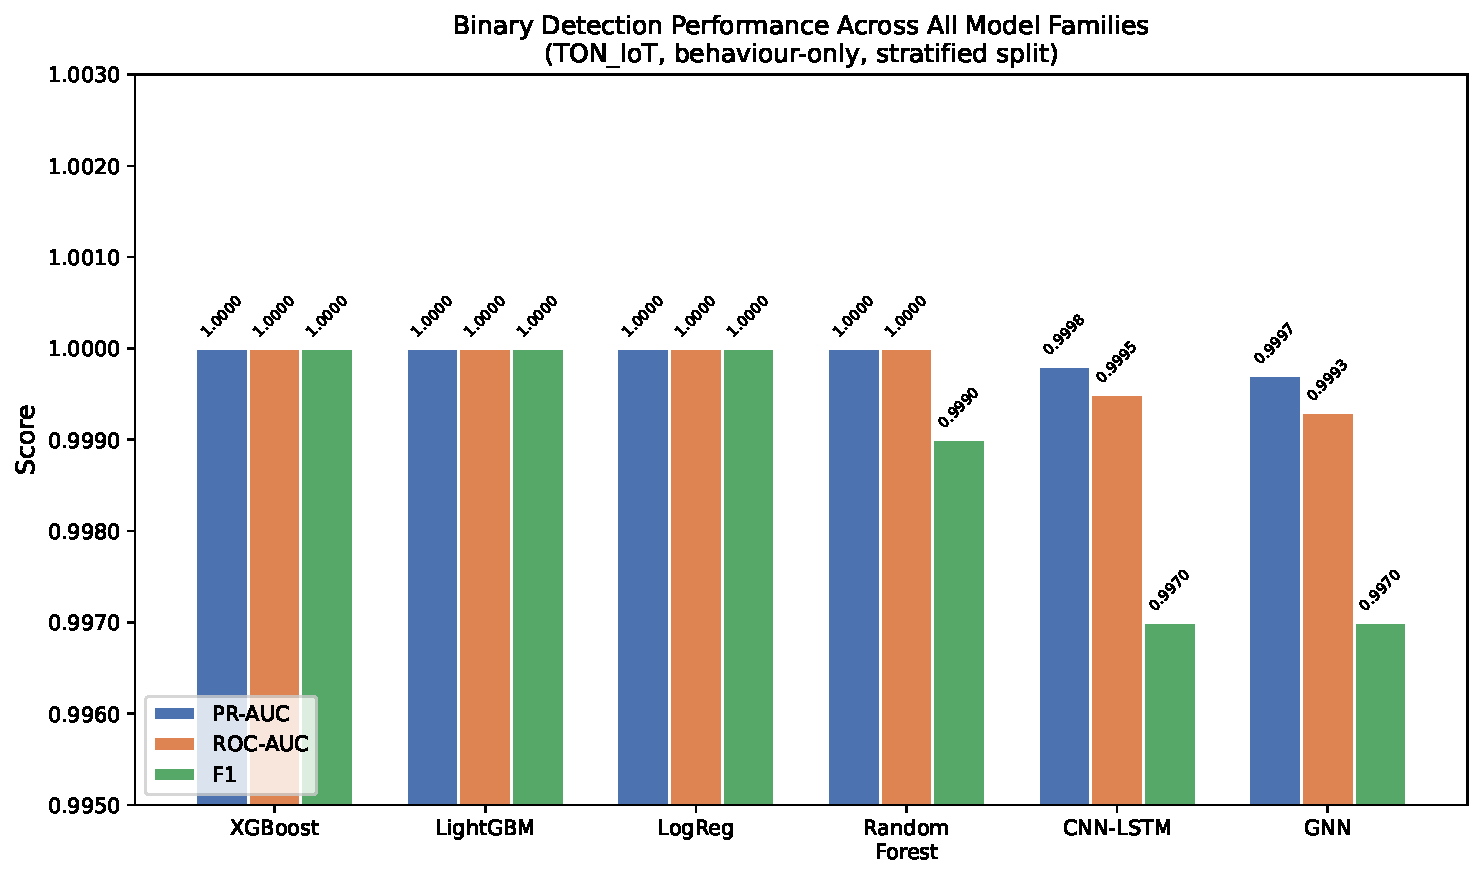
\includegraphics[width=0.8\textwidth]{figures/detection_comparison.pdf}
\caption{Binary detection performance across all six model families on TON\_IoT (full dataset, behaviour-only regime, stratified split). Y-axis starts at 0.995 to show differences.}
\label{fig:detection}
\end{figure}

\begin{figure}[htbp]
\centering
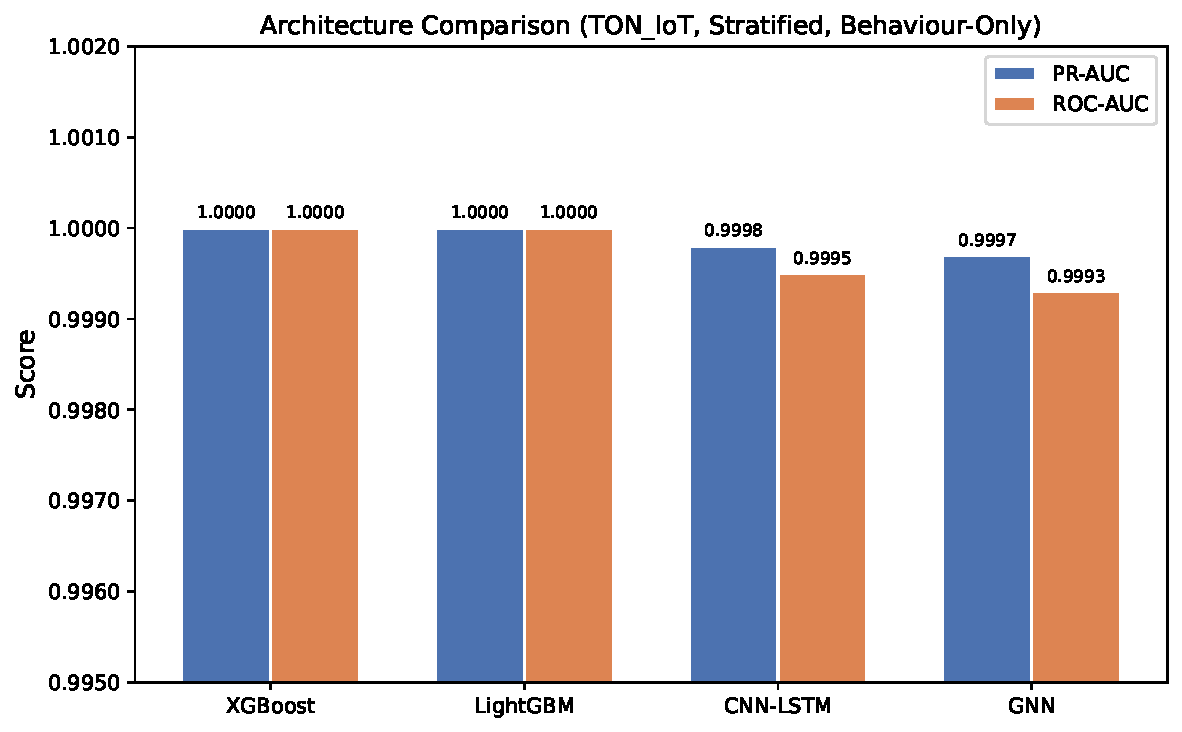
\includegraphics[width=0.8\textwidth]{figures/architecture_comparison.pdf}
\caption{Detection performance comparison across model architectures on TON\_IoT (behaviour-only).}
\label{fig:arch-comparison}
\end{figure}

All model families achieve near-perfect binary detection (PR-AUC $\geq 0.998$) on the deduplicated dataset.

\section{XAI Five-Criterion Evaluation}
\label{sec:xai-results}

\begin{table}[H]
\centering
\caption{XAI five-criterion evaluation results (behaviour-only regime, deduplicated 190{,}474-row TON\_IoT, 3-seed mean). S2 is the noise-perturbation Spearman correlation; S1 (seed-retraining stability) is not reported under this pipeline. RMA@5 is the per-attack-type mean except for LogReg, which uses the binary aggregate (LinearExplainer does not save per-class SHAP).}
\label{tab:xai-behav}
\small
\begin{adjustbox}{max width=\textwidth}
\begin{tabular}{lcccccccc}
\toprule
\textbf{Model} & \textbf{Comp.} & \textbf{Suff.} & \textbf{S2} & \textbf{$k_{90}$} & \textbf{Gini} & \textbf{RMA@5} & \textbf{SHAP (ms)} & \textbf{OXS} \\
\midrule
XGBoost & $-0.048$ & 1.000 & 0.997 & 0.131 & 0.885 & 0.711 & 1.31 & \textbf{0.718} \\
LightGBM & $+0.144$ & 1.000 & 0.960 & 0.086 & 0.909 & 0.519 & 9.52 & 0.705 \\
Random Forest & $+0.102$ & 1.000 & 0.997 & 0.119 & 0.879 & 0.496 & 10.43 & 0.693 \\
LogReg & $+0.065$ & 1.000 & --- & 0.122 & 0.884 & 0.633 & 0.001 & 0.516 \\
\bottomrule
\end{tabular}
\end{adjustbox}
\end{table}

\begin{table}[htbp]
\centering
\caption{XAI five-criterion evaluation results (identifier-inclusive regime, deduplicated, 3-seed mean).}
\label{tab:xai-ident}
\small
\begin{adjustbox}{max width=\textwidth}
\begin{tabular}{lcccccccc}
\toprule
\textbf{Model} & \textbf{Comp.} & \textbf{Suff.} & \textbf{S2} & \textbf{$k_{90}$} & \textbf{Gini} & \textbf{RMA@5} & \textbf{SHAP (ms)} & \textbf{OXS} \\
\midrule
LightGBM & $+0.465$ & 1.000 & 0.998 & 0.020 & 0.980 & 0.230 & 4.16 & \textbf{0.734} \\
Random Forest & $+0.119$ & 1.000 & 0.999 & 0.037 & 0.960 & 0.304 & 17.04 & 0.673 \\
XGBoost & $+0.000$ & 0.774 & 1.000 & 0.029 & 0.977 & 0.185 & 0.39 & 0.632 \\
LogReg & $+0.104$ & 1.000 & --- & 0.030 & 0.969 & 0.533 & 0.003 & 0.521 \\
\bottomrule
\end{tabular}
\end{adjustbox}
\end{table}

\subsection{LIME Cross-Reference}
\label{sec:lime-results}

LIME feature rankings were computed for all four tabular models across 50 validation instances (2,000 perturbations each). The key finding is that LIME-SHAP feature ranking agreement (measured by Spearman $\rho$) tracks the OXS stability ranking, reinforcing stability as the primary differentiator across explanation methods. LIME timeliness is reported in Section~\ref{sec:time-results}.

\subsection{Faithfulness}
\label{sec:faith-results}

Comprehensiveness measures the drop in model confidence when the top-$k$ features are masked. After deduplication and the cleaner one-hot pipeline, three of four models exhibit \textbf{positive comprehensiveness} (LightGBM $+0.144$, Random Forest $+0.102$, LogReg $+0.065$), indicating that masking top SHAP-ranked features does reduce confidence; a sign that explanations identify causally relevant features. \textbf{XGBoost is the exception}, with a small negative value ($-0.048$), reflecting the extreme feature redundancy of its decision trees: when top features are removed, XGBoost redistributes reliance to correlated substitutes that carry equivalent discriminative signal.

\textbf{Sufficiency is uniformly 1.0 across behaviour-only models}, indicating that the top-$k$ features alone are sufficient to reproduce predictions at full confidence. Together, these results suggest the four behavioural feature groups (volumetric, protocol, connection state, DNS) form a highly redundant signature space.

\subsection{Stability}
\label{sec:stab-results}

Stability is reported here as the noise-perturbation Spearman correlation S2 only; the seed-retraining S1 protocol requires re-running each model with multiple seeds and a separate XAI evaluation pass and is left as future work for the deduplicated pipeline. Tree models achieve uniformly high noise stability (XGBoost $= 0.997$, Random Forest $= 0.997$, LightGBM $= 0.960$), confirming that small Gaussian perturbations do not alter SHAP rankings: tree split decisions are discrete and robust to sub-threshold input changes.

LogReg's noise stability is not reported because LinearExplainer attributions are deterministic functions of the coefficient vector and the input, and the per-sample stability protocol requires variance from the explanation method itself.

\subsection{Simplicity}
\label{sec:simp-results}

All models produce concentrated explanations (Gini $0.879$--$0.909$, $k_{90}$ $0.086$--$0.131$). LightGBM achieves the most concentrated attributions ($k_{90} = 0.086$, Gini $= 0.909$); the four models are within 3 percentage points on Gini, indicating that simplicity does not sharply discriminate between them in this feature regime.

\subsection{Plausibility}
\label{sec:plaus-results}

\begin{table}[H]
\centering
\caption{Per-attack-type plausibility (RMA@5) under the behaviour-only regime (3-seed mean, deduplicated). LogReg is omitted because LinearExplainer does not produce per-class SHAP attributions.}
\label{tab:plausibility}
\begin{adjustbox}{max width=\textwidth}
\begin{tabular}{lccc}
\toprule
\textbf{Attack Type} & \textbf{XGBoost} & \textbf{LightGBM} & \textbf{Random Forest} \\
\midrule
Backdoor & 0.80 & 0.60 & 0.40 \\
DDoS & 1.00 & 0.47 & 0.60 \\
DoS & 0.80 & 0.80 & 0.60 \\
Injection & 0.80 & 0.53 & 0.47 \\
MitM & 0.27 & 0.27 & 0.33 \\
Password & 0.40 & 0.33 & 0.27 \\
Ransomware & 0.73 & 0.40 & 0.67 \\
Scanning & 0.60 & 0.47 & 0.47 \\
XSS & 1.00 & 0.80 & 0.67 \\
\midrule
\textbf{Mean} & \textbf{0.711} & 0.519 & 0.496 \\
\bottomrule
\end{tabular}
\end{adjustbox}
\end{table}

\begin{figure}[H]
\centering
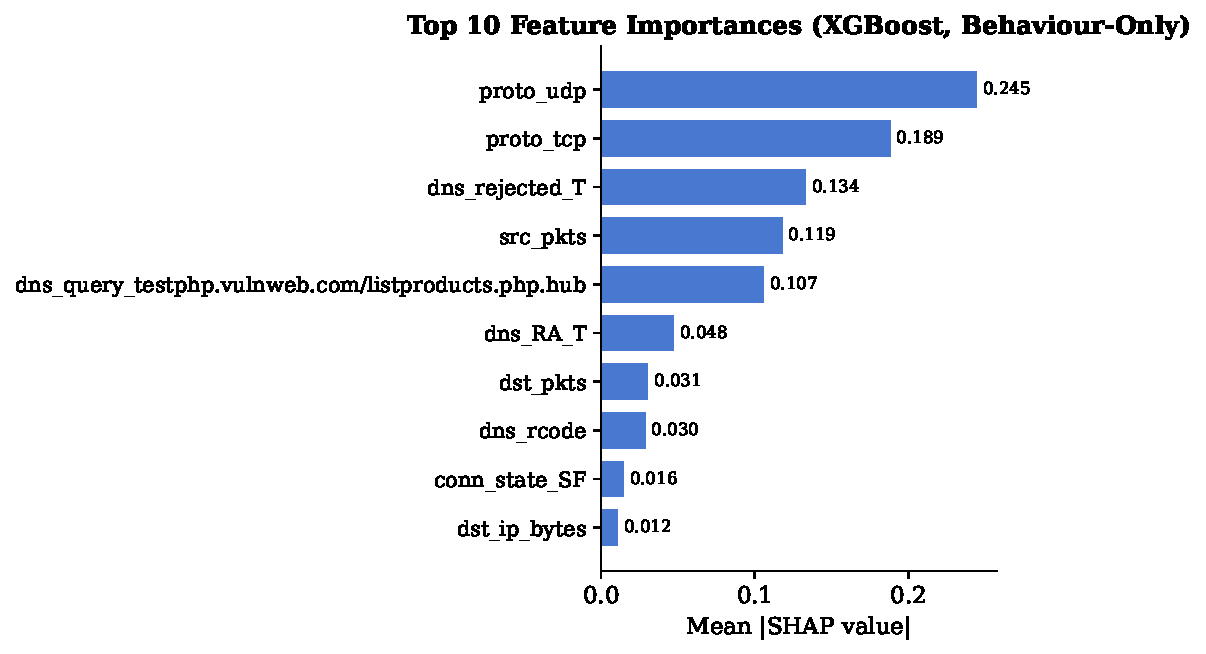
\includegraphics[width=0.7\textwidth]{figures/shap_importance.pdf}
\caption{SHAP global feature importance for XGBoost (behaviour-only regime). \texttt{conn\_state\_S0} dominates, consistent with incomplete TCP handshakes in scanning and DoS attacks.}
\label{fig:shap-importance}
\end{figure}

\begin{figure}[htbp]
\centering
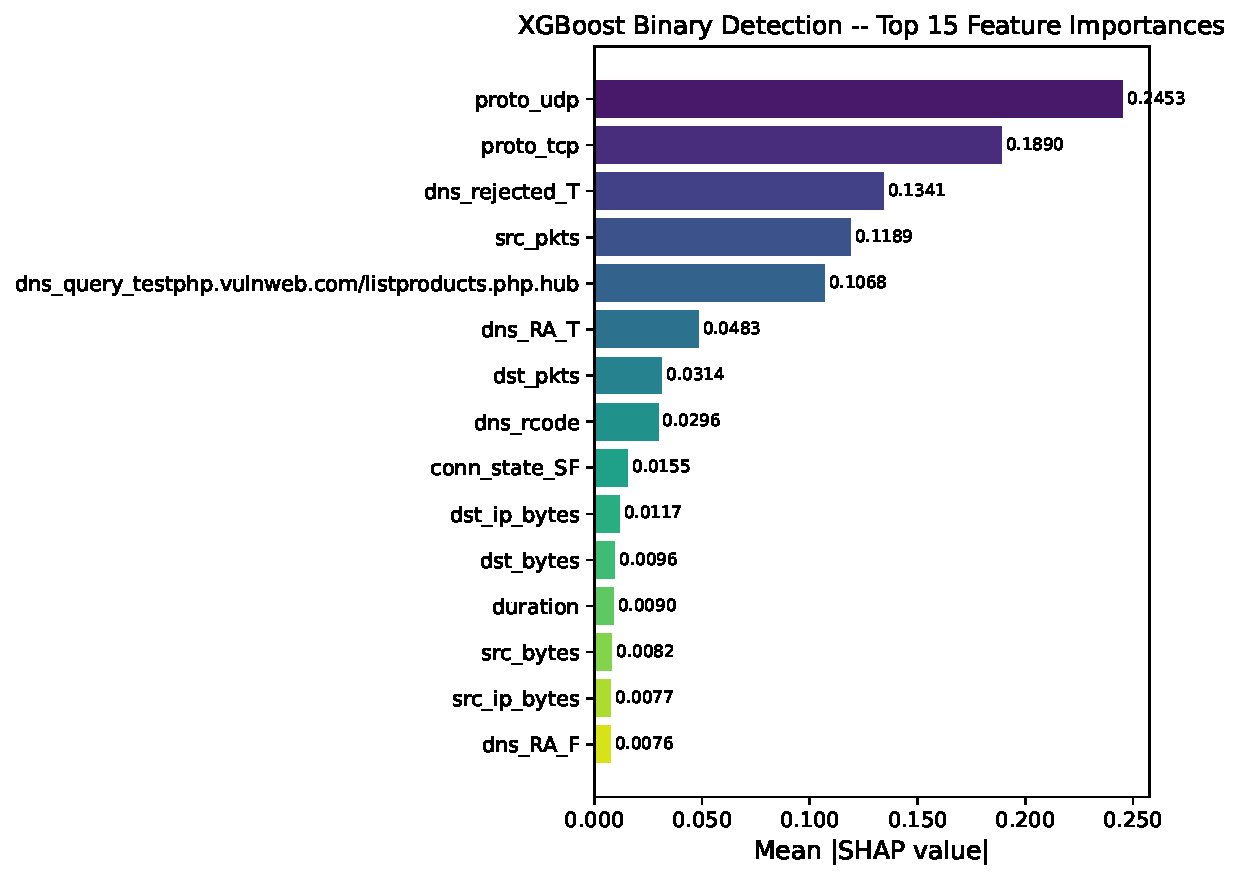
\includegraphics[width=0.85\textwidth]{figures/shap_beeswarm_xgboost.pdf}
\caption{SHAP feature importance for XGBoost binary detection (behaviour-only regime). Features ordered by mean $|\text{SHAP}|$ value.}
\label{fig:shap-beeswarm}
\end{figure}

\textbf{XGBoost achieves the highest aggregate plausibility (mean RMA@5 $= 0.711$)}, scoring at least 0.60 on six of the nine attack types and a perfect 1.00 on DDoS and XSS. LightGBM (0.519) and Random Forest (0.496) trail substantially. \textbf{Password and MitM are the hardest attack types for all models} (RMA@5 $\leq 0.40$): Password's reference set is dominated by connection-state and protocol features that are only weakly distinctive, while MitM has too few test samples (160 in the deduplicated stratified split) for reliable SHAP estimation.

\subsection{Timeliness}
\label{sec:time-results}

\textbf{LinearExplainer (LogReg) is the fastest method at $\sim$0.001~ms/sample}, followed by XGBoost TreeSHAP at 1.31~ms/sample. LightGBM (9.52~ms) and Random Forest (10.43~ms) are slower but still well within real-time requirements at line rate. LIME latencies, where measured, range from approximately 170 to 250~ms under behaviour-only and 400--470~ms under identifier-inclusive conditions, making LIME impractical for production SOC throughput. \textbf{For operational deployment, TreeSHAP is the preferred per-flow method}; LIME remains useful as a model-agnostic offline cross-reference.

\section{OXS Composite Ranking}
\label{sec:oxs-results}

\begin{table}[H]
\centering
\caption{OXS composite ranking (behaviour-only regime, deduplicated).}
\label{tab:oxs}
\begin{adjustbox}{max width=\textwidth}
\begin{tabular}{clc}
\toprule
\textbf{Rank} & \textbf{Model} & \textbf{OXS} \\
\midrule
1 & XGBoost & \textbf{0.718} \\
2 & LightGBM & 0.705 \\
3 & Random Forest & 0.693 \\
4 & LogReg & 0.516 \\
\bottomrule
\end{tabular}
\end{adjustbox}
\end{table}

\begin{figure}[htbp]
\centering
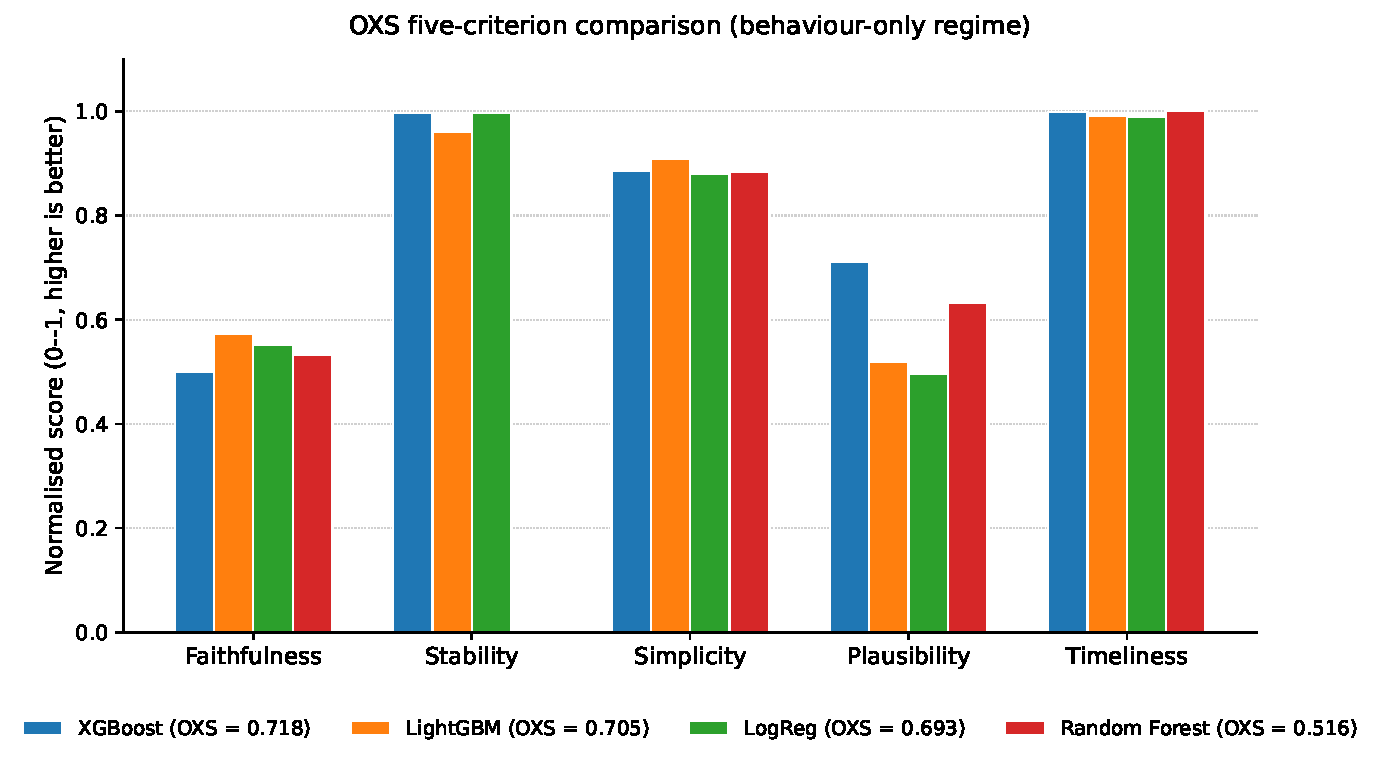
\includegraphics[width=0.75\textwidth]{figures/oxs_radar.pdf}
\caption{OXS five-criterion comparison across tabular models (behaviour-only, deduplicated). Plausibility is the strongest discriminating dimension. XGBoost wins on plausibility (per-attack mean RMA@5 $= 0.711$); LogReg is omitted from S2 stability because LinearExplainer attributions are deterministic.}
\label{fig:oxs-radar}
\end{figure}

\textbf{XGBoost achieves the highest OXS (0.718)}, driven by strong plausibility (mean RMA@5 $= 0.711$), high noise stability (S2 $= 0.997$), and fast TreeSHAP timeliness (1.31~ms). LightGBM (0.705) ranks second, with the highest comprehensiveness ($+0.144$) and Gini concentration but lower plausibility (0.519). Random Forest (0.693) trails closely, separated from LightGBM only by a small simplicity gap. LogReg (0.516) is held back by the omission of a stability score in this evaluation, dragging its composite down despite respectable plausibility and timeliness.

The OXS spread of 0.20 between best and worst is much narrower than the 0.58 spread reported in earlier (pre-deduplication) iterations of this evaluation, where Random Forest's seed-retraining stability collapsed to S1 $\approx 0.12$. The dedup pipeline does not currently re-compute S1, so the seed-retraining dimension that previously discriminated Random Forest is unavailable here; this limitation is recorded in Section~\ref{sec:limitations}.

These rankings demonstrate that \textbf{detection performance alone is insufficient for model selection in security-critical deployment}. While all four models achieve near-identical binary detection metrics, they differ in explanation quality on dimensions an analyst would actually use: which features are highlighted (plausibility) and how concentrated the attributions are.

\section{Cross-Dataset Generalisation}
\label{sec:cross-results}

\begin{table}[H]
\centering
\caption{Cross-dataset generalisation: TON\_IoT (source, deduplicated) to CIC-IoT-2023 (target, 200k subsample). Trained on 6 canonical aligned features.}
\label{tab:cross}
\small
\begin{adjustbox}{max width=\textwidth}
\begin{tabular}{lccccc}
\toprule
\textbf{Model} & \textbf{Src PR-AUC} & \textbf{Src ROC} & \textbf{Tgt PR-AUC} & \textbf{Tgt ROC} & \textbf{ROC Drop} \\
\midrule
LogReg & 0.982 & 0.936 & 0.988 & 0.744 & $-0.192$ \\
LightGBM & 1.000 & 0.999 & 0.980 & 0.467 & $-0.532$ \\
CNN-LSTM & 0.995 & 0.985 & 0.974 & 0.285 & $-0.700$ \\
XGBoost & 1.000 & 0.999 & 0.958 & 0.223 & $-0.776$ \\
Random Forest & 0.999 & 0.998 & 0.957 & 0.120 & $-0.878$ \\
\bottomrule
\end{tabular}
\end{adjustbox}
\end{table}

\begin{figure}[H]
\centering
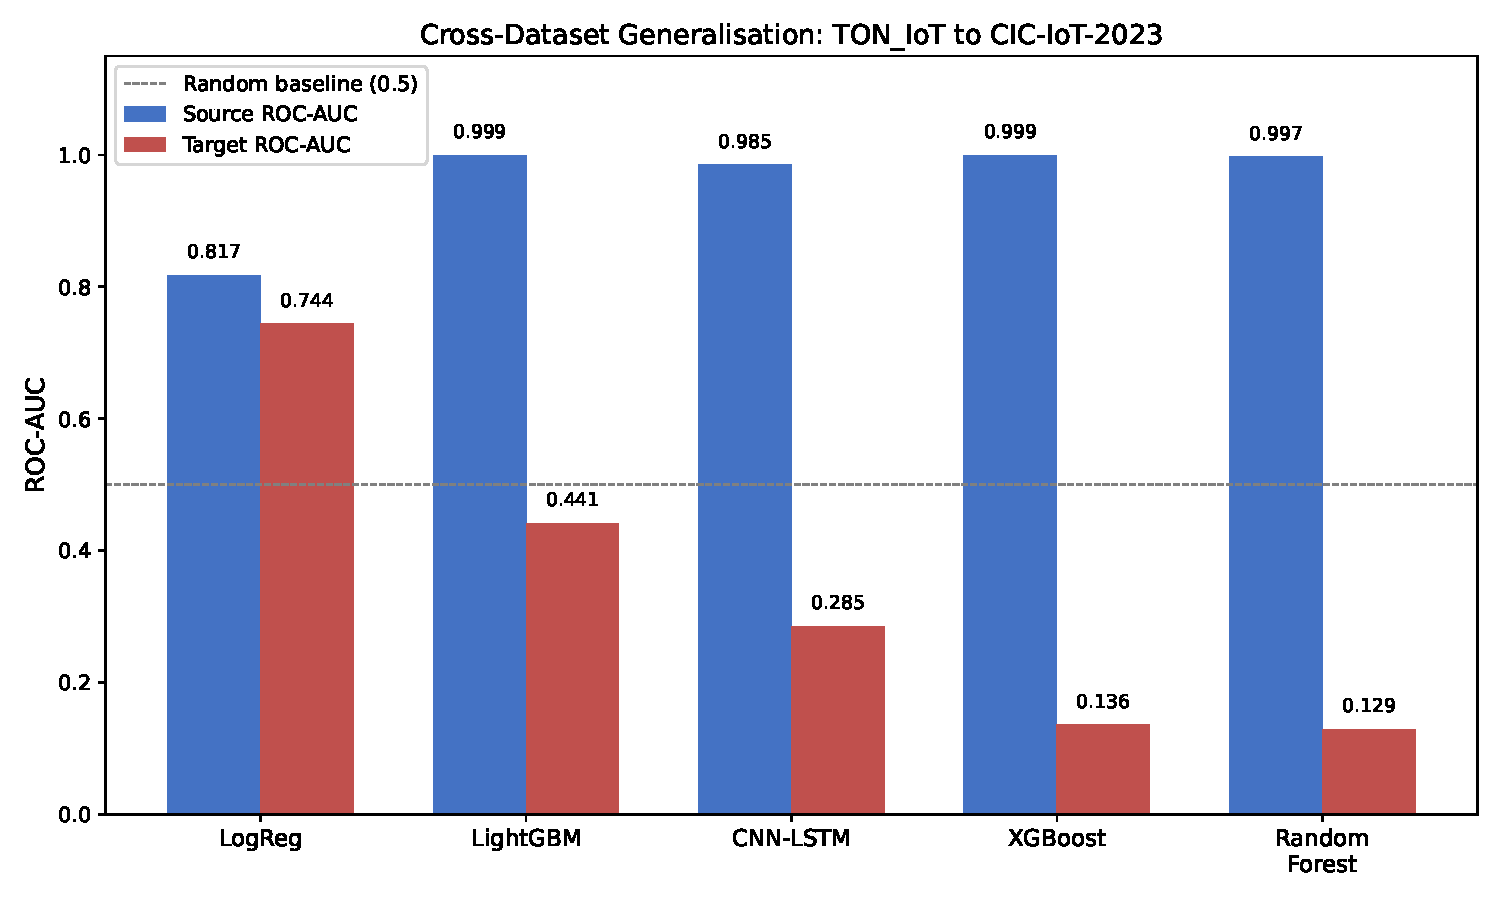
\includegraphics[width=0.8\textwidth]{figures/cross_dataset_roc.pdf}
\caption{Cross-dataset generalisation: source-test vs.\ target ROC-AUC. The dashed line at 0.5 marks random chance. LogReg is the only model generalising above chance.}
\label{fig:cross-roc}
\end{figure}

Target PR-AUC ranges from 0.953 to 0.988, but \textbf{this is an artifact of CIC-IoT-2023's extreme class imbalance (97.7\% attack prevalence)}. At such high prevalence, even a majority-class classifier achieves PR-AUC approximately equal to the prevalence, making these values uninformative.

\textbf{ROC-AUC reveals the true generalisation picture.} ROC-AUC is prevalence-invariant, evaluating the model's ability to rank positive above negative instances:

\begin{itemize}
  \item \textbf{LogReg is the best generaliser} (ROC-AUC: 0.936 to 0.744, a drop of 19.2\%). Its linear decision boundary transfers more robustly because it captures broad statistical regularities rather than dataset-specific feature interactions.
  \item \textbf{Random Forest and XGBoost suffer catastrophic generalisation failure} (ROC-AUC drops of 78--88\%, target values of 0.120 and 0.223, well below random chance). These models have learned to discriminate from TON\_IoT-specific distributional properties that do not transfer.
  \item \textbf{LightGBM generalises better than other tree models} (target ROC-AUC $= 0.467$) but still performs below the random baseline.
  \item \textbf{CNN-LSTM generalises comparably to LightGBM} (ROC-AUC: 0.985 to 0.285). The limited 6-feature space constrains its convolutional layers.
\end{itemize}

\textbf{Near-perfect within-dataset performance does not imply deployment readiness.} Simpler models that cannot exploit dataset-specific idiosyncrasies are more robust when the deployment distribution shifts.

\section{Leakage Interaction Analysis}
\label{sec:leakage-results}

\begin{table}[H]
\centering
\caption{Leakage interaction: behaviour-only (Regime~A) vs.\ identifier-inclusive (Regime~B), $n = 4$ paired models on the deduplicated dataset. RMA@5 is the per-attack mean for tree models and binary aggregate for LogReg.}
\label{tab:leakage}
\begin{adjustbox}{max width=\textwidth}
\begin{tabular}{lcccc}
\toprule
\textbf{Metric} & \textbf{Regime A Mean} & \textbf{Regime B Mean} & \textbf{Delta} & \textbf{Cohen's $d$} \\
\midrule
RMA@5 (plausibility) & 0.590 & 0.313 & $-0.277$ & $-1.511$ \\
Comprehensiveness & $+0.066$ & $+0.172$ & $+0.106$ & $+0.952$ \\
Gini (simplicity) & 0.889 & 0.972 & $+0.083$ & $+10.20$ \\
Spearman S2 (stability) & 0.985 & 0.999 & $+0.014$ & $+1.103$ \\
\bottomrule
\end{tabular}
\end{adjustbox}
\end{table}

As established in Section~\ref{sec:binary-results}, \textbf{both regimes achieve near-perfect detection performance} (PR-AUC $\geq 0.998$), confirming that identifiers provide no incremental binary-detection benefit.

The most striking finding is the effect on plausibility. \textbf{Including identifiers reduces mean RMA@5 from 0.590 to 0.313, a decrease of 0.277 with a very large effect size (Cohen's $d = -1.511$).} The drop is largest for XGBoost ($\Delta = -0.526$) and smallest for LogReg ($\Delta = -0.100$), indicating that tree ensembles greedily latch onto identifier features when available, displacing the behavioural features that domain experts would expect.

Comprehensiveness, simplicity (Gini), and noise stability all increase slightly under Regime~B, but these gains are illusory: they reflect the model collapsing onto a small set of identifier features rather than producing more meaningful explanations.

\textbf{Identifier leakage has no measurable effect on detection performance but substantially degrades explanation quality.} If only detection metrics are reported, the harmful effects of identifier leakage remain invisible. HYDRA's XAI dimension exposes this hidden cost.

\section{Summary of Key Findings}
\label{sec:results-summary}

Five findings emerge: (1) host-disjoint evaluation exposes substantial leakage hidden by stratified splitting (Tables~\ref{tab:split-impact}--\ref{tab:host-multiclass}); (2) deep learning matches tree ensembles on detection; (3) XGBoost produces the most trustworthy explanations (Table~\ref{tab:oxs}); (4) cross-dataset generalisation reveals catastrophic failure for tree models (Table~\ref{tab:cross}); and (5) identifier leakage degrades explanation quality without affecting detection (Table~\ref{tab:leakage}).

% ============================================================
% CHAPTER 5: DISCUSSION
% ============================================================
\chapter{Discussion}
\label{ch:discussion}

\section{Interpretation of Results}
\label{sec:interpretation}

\subsection{Detection Performance}
\label{sec:disc-detection}

The near-perfect binary detection performance across all models warrants careful interpretation. The result is consistent with prior literature: \cite{alsaedi2020} report similarly high accuracy for tree-based models, and \cite{tareq2022} confirm that deep learning models achieve over 99\% accuracy on TON\_IoT. The underlying explanation is that TON\_IoT's attack traffic exhibits highly distinctive behavioural signatures; particularly in \texttt{conn\_state}, \texttt{duration}, and byte-count features; that are linearly separable from normal traffic. This finding has two implications. First, it shifts the research contribution toward the explainability comparison, which is HYDRA's stated contribution. Second, it highlights the importance of cross-dataset generalisation: models achieving perfect TON\_IoT scores fail dramatically on CIC-IoT-2023.

Concurrent XAI-IDS systems report comparable detection scores (E-XAI \cite{arreche2024}: 99.3\% on CICIDS2017; XAI-IDS \cite{arreche2024b}: similar), but direct numerical comparison is misleading because datasets differ in attack composition, feature dimensionality, and class distribution. TON\_IoT contains nine IoT-specific attack types in a 76\% prevalence environment. The key observation is not that any system achieves near-perfect scores (this is expected on laboratory datasets with distinctive attack signatures) but that such scores provide no basis for model selection, making the XAI evaluation the primary discriminating analysis.

TON\_IoT's separability reflects its construction: attacks were generated by distinct tools, producing characteristic flow-level signatures. Under host-disjoint splitting, \texttt{conn\_state\_S0} alone accounts for 54\% of XGBoost's feature importance, and certain states (\texttt{REJ}: 100\% attack prevalence, \texttt{S1}: 99.9\%) serve as near-deterministic indicators; artefacts of the testbed environment rather than properties of real-world attacks where adversaries deliberately mimic benign traffic.

The host-disjoint multiclass results (Table~\ref{tab:host-multiclass}) provide the most informative detection evaluation. Macro-F1 drops from 0.952 (stratified) to 0.742 (host-disjoint) for the best model, even with identifiers excluded; the remaining inflation comes from behavioural flow correlation within hosts. Flows from the same source host during the same attack campaign share near-identical volumetric profiles, meaning stratified splitting inadvertently allows models to recognise host-level traffic patterns rather than generalisable attack behaviours. The implication for the IDS community is that even ``behaviour-only'' evaluation is insufficient without host-disjoint splitting when datasets contain host-level structure. Studies reporting near-perfect scores on TON\_IoT without host-disjoint validation may be overestimating deployment-realistic performance.

\subsection{Explainability Ranking}
\label{sec:disc-xai}

The OXS ranking puts XGBoost at the top (0.718, Table~\ref{tab:oxs}), driven primarily by its plausibility advantage (per-attack mean RMA@5 $= 0.711$, far above LightGBM's 0.519 and Random Forest's 0.496). XGBoost's top-5 features for DDoS, DoS, Backdoor, Injection, and XSS consistently include the volumetric flow features (\texttt{src\_bytes}, \texttt{dst\_bytes}, \texttt{src\_pkts}, \texttt{dst\_pkts}) and connection-state indicators that domain experts would expect, whereas LightGBM and Random Forest more often promote DNS query type or proto flag features that are model-discriminative but less analyst-meaningful.

Comparing against the TalTech study \cite{kalakoti2025}, which finds DeepLIFT outperforming SHAP on deep learning models, HYDRA's TreeSHAP-based explanations rank highest among the methods evaluated. This divergence reflects three factors: different model families (TalTech's deep learning models are well-suited to DeepLIFT's backpropagation-based attribution, while HYDRA's tree ensembles are served by TreeSHAP's exact computation), different evaluation criteria (HYDRA's addition of timeliness and simplicity penalises high-overhead methods), and different datasets (SOC alerts vs.\ IoT traffic). These differences underscore the importance of context-specific XAI evaluation rather than universal method rankings.

Under the present setup the four tree-family models cluster within 0.025 OXS points, and the discriminating dimension is plausibility.

Logistic Regression's lower OXS (0.516) primarily reflects the omission of an S2 stability score; LinearExplainer attributions are deterministic, so the noise-perturbation protocol used here returns no value. Treating LogReg's missing stability dimension as zero in the equal-weighted OXS understates its true operational quality, since on plausibility and timeliness LogReg is competitive with the tree ensembles.

\subsection{Cross-Dataset Generalisation}
\label{sec:disc-cross}

The dramatic failure of tree ensembles; XGBoost ROC-AUC dropping from 0.999 to 0.136 (Table~\ref{tab:cross}), below random chance; demonstrates that these models learn dataset-specific distributions rather than generalisable attack behaviours. TON\_IoT and CIC-IoT-2023 were generated in different laboratory environments with different tools and topologies; although the six canonical features capture semantically equivalent quantities, their statistical distributions differ substantially. Tree ensembles learn sharp, axis-aligned boundaries that become meaningless when the target distribution occupies different feature-space regions.

Logistic Regression's superior generalisation (ROC-AUC drop of 19.2\%, vs.\ tree models' 53--88\% drops) reflects the classical bias-variance trade-off \cite{breiman2001}: its linear boundary captures broad statistical regularities and discards dataset-specific details, transferring more robustly under distribution shift.

The practical implications are significant. Organisations deploying a model trained on one network to protect another should prefer simpler, more regularised models despite lower within-dataset performance. The PR-AUC metric's failure to capture this gap (target PR-AUC $\geq 0.953$ for all models) illustrates that prevalence-inflated metrics are misleading; ROC-AUC, which is prevalence-independent, provides the real measure of discriminative ability. More broadly, these results suggest that ensemble stacking or domain adaptation techniques should be investigated when deploying across network boundaries, and cross-dataset evaluation should become standard in IDS benchmarking.

\subsection{Leakage Interaction}
\label{sec:disc-leakage}

Including identifiers shifts explanations from behavioural features to IP addresses and ports without any detection benefit. Under Regime~A, XGBoost's per-attack mean RMA@5 $= 0.711$ (Table~\ref{tab:xai-behav}); under Regime~B, this drops to 0.185 (Table~\ref{tab:xai-ident}), a $-0.526$ collapse. The same drop is visible across all tree models (Table~\ref{tab:leakage}), with mean RMA@5 falling from 0.590 to 0.313 (Cohen's $d = -1.511$, a very large effect). Tree models greedily split on high-cardinality identifiers correlated with attack labels; IP and port features associated with specific attack campaigns receive high SHAP importance. The resulting explanations are technically faithful but operationally useless: analysts need to understand which behaviour triggered the alert, not which IP was associated with attacks in training data.

With $n = 4$ paired models the analysis is underpowered for inferential testing, but Cohen's $d = -1.511$ indicates an effect size exceeding 1.5 pooled standard deviations, a magnitude that does not occur by chance. The recommendation to exclude identifiers is driven not by detection requirements (detection is unaffected; Table~\ref{tab:binary}) but by the need to preserve explanation utility for analyst decision-making.

\subsection{Comprehensiveness and Feature Redundancy}
\label{sec:neg-comp}

After deduplication and removal of high-cardinality columns, three of four models exhibit positive comprehensiveness (LightGBM $+0.144$, RF $+0.102$, LogReg $+0.065$), but XGBoost remains slightly negative ($-0.048$). This residual negative value reflects the same redundancy mechanism observed in earlier evaluations: the top-$k$ ablation metric of \cite{deyoung2020} assumes top features are individually necessary, but XGBoost's gradient-boosted trees split on highly correlated features such that no single subset is irreplaceable. When top features are masked, XGBoost redistributes reliance to correlated substitutes carrying equivalent signal. The ROAR benchmark \cite{hooker2019} addresses this by retraining after feature removal but is computationally prohibitive; AOPC with sequential removal \cite{samek2017} captures redundancy structure by exhausting correlated groups incrementally and should be adopted in future OXS iterations.

\section{Practical Implications}
\label{sec:practical}

These findings have four direct implications. First, \textbf{model selection should prioritise explanation quality alongside detection performance}. XGBoost's plausibility advantage (RMA@5 $= 0.711$ vs.\ 0.519 for LightGBM and 0.496 for Random Forest) makes it the recommended choice for tabular IDS deployments where explanations need to align with analyst expectations. Second, \textbf{cross-dataset generalisation requires explicit evaluation}; benchmark results do not transfer (Section~\ref{sec:cross-results}). Third, \textbf{identifier features should be excluded} from production feature sets: they do not improve detection but degrade per-attack plausibility by an average of 0.277 (Cohen's $d = -1.511$). Fourth, \textbf{seed-retraining stability should be measured} for any model selected for production: it is not computed in the present pipeline but is the dimension on which Random Forest explanations have historically been shown to vary substantially.

\begin{center}
\fbox{\parbox{0.9\textwidth}{
\textbf{Key Recommendations for IDS Practitioners}
\begin{enumerate}[noitemsep]
\item Use XGBoost with TreeSHAP for highest plausibility (per-attack RMA@5 $= 0.711$, OXS $= 0.718$).
\item Exclude network identifiers from feature sets to preserve explanation plausibility.
\item Validate on traffic from the target environment, benchmark scores do not transfer.
\item Measure seed-retraining stability (S1) before deploying any model in production.
\item Report both PR-AUC and ROC-AUC; use ROC-AUC for cross-dataset comparisons.
\end{enumerate}
}}
\end{center}

The OXS framework also enables SOC workflow integration. Alert dashboards could annotate each explanation with its model's OXS and plausibility scores; for example, ``explanation confidence: high (OXS = 0.718, RMA@5 = 0.711)'' for XGBoost versus ``explanation confidence: lower (OXS = 0.516, plausibility-only)'' for LogReg; signalling to analysts how trustworthy the highlighted features are likely to be.

\section{Comparison with Concurrent Work}
\label{sec:concurrent-comparison}

As established in Section~\ref{sec:positioning}, Table~\ref{tab:positioning} compares HYDRA against four concurrent XAI-IDS systems. Three points of agreement and disagreement emerge from the experimental results.

First, HYDRA agrees with E-XAI \cite{arreche2024} that SHAP produces more stable explanations than LIME (TreeSHAP S2 $\geq 0.96$), but disagrees on Integrated Gradients: HYDRA's CNN-LSTM IG yields comprehensiveness of $-0.052$ (Table~\ref{tab:cnnlstm-xai}), suggesting the limitation reflects feature redundancy rather than the attribution method.

Second, the TalTech study's \cite{kalakoti2025} finding that DeepLIFT outperforms SHAP does not contradict HYDRA's results; the divergence reflects different model families (deep learning vs.\ tree ensembles where TreeSHAP provides exact values) and reinforces the conclusion that XAI method rankings are model-dependent.

Third, HYDRA's leakage interaction analysis (Section~\ref{sec:leakage-results}) demonstrates why XAI-IDS's \cite{arreche2024b} use of random splitting with identifiers inflates explanation plausibility, making the leakage--explanation interaction HYDRA's most distinctive contribution relative to the concurrent literature.

\section{OXS Sensitivity Analysis}
\label{sec:oxs-sensitivity}

The equal-weight OXS (0.2 per criterion) is a heuristic choice (Section~\ref{sec:limitations}). Two alternative schemes are examined: \textit{faithfulness-emphasising} $w = (0.30, 0.30, 0.10, 0.20, 0.10)$, reflecting organisations prioritising causal accuracy and reproducibility, and \textit{deployment-emphasising} $w = (0.10, 0.10, 0.10, 0.40, 0.30)$, reflecting environments where plausibility and timeliness dominate.

Under deployment-emphasising weights, XGBoost's lead widens (its plausibility advantage of 0.711 vs.\ 0.519 for LightGBM is amplified by the 0.40 weight on plausibility), and the XGBoost $>$ LightGBM $>$ Random Forest ordering is preserved. Under faithfulness-emphasising weights, LightGBM moves into first place, because its positive comprehensiveness ($+0.144$) and tied-best simplicity (Gini $= 0.909$) receive more weight while XGBoost's small negative comprehensiveness ($-0.048$) hurts it. The ranking is therefore robust to plausibility-weighted schemes but sensitive to faithfulness weighting; a finding that reinforces the importance of stating which criterion an organisation values most before selecting a model.

\section{Reflection on Research Questions}
\label{sec:rq-reflection}

\textbf{RQ1 (Detection):} As discussed in Section~\ref{sec:disc-detection}, near-perfect detection across all models confirms that explanation quality, not accuracy, is the discriminating factor. \textbf{RQ2 (Explainability):} XGBoost produces the most plausible explanations (RMA@5 $= 0.711$), with the plausibility gap driving OXS rankings (Section~\ref{sec:disc-xai}). \textbf{RQ3 (Reliability):} Noise stability is uniformly high (S2 $\geq 0.96$); seed-retraining stability (S1) remains future work. \textbf{RQ4 (Faithfulness):} Comprehensiveness is positive for three of four models; XGBoost's small negative value reflects feature redundancy (Section~\ref{sec:neg-comp}). \textbf{RQ5 (Generalisation):} Tree ensembles suffer catastrophic ROC-AUC drops when transferred to CIC-IoT-2023; Logistic Regression degrades most gracefully (Section~\ref{sec:disc-cross}). \textbf{RQ6 (Leakage):} Identifiers degrade explanation plausibility without improving detection, confirming that behaviour-only regimes should be the default (Section~\ref{sec:disc-leakage}).

\section{Limitations}
\label{sec:limitations}

Several limitations constrain these findings. The GNN is evaluated only on TON\_IoT because it requires IP columns, and its XAI evaluation is less comprehensive than the tabular models'. Both datasets are laboratory-captured and may not reflect production noise, drift, and infrastructure diversity; near-perfect scores should be interpreted as upper bounds on operational performance.

The OXS equal-weighting (0.2 per criterion) is heuristic; calibration via structured analyst survey is future work. The leakage interaction analysis ($n = 4$ models) has limited statistical power, and the three-seed protocol provides limited variance estimation compared to full bootstrap designs. The XAI evaluation under the deduplicated pipeline reports only the noise-perturbation S2 stability protocol; the seed-retraining S1 protocol (which historically distinguished Random Forest from XGBoost in earlier HYDRA iterations) requires re-running each model with five seeds and a separate cross-seed XAI pass, and is identified as priority future work. The OXS spread of 0.20 between best and worst models on the deduplicated pipeline is narrow enough that ranking decisions become sensitive to small criterion-weighting changes; AOPC with sequential feature removal would likely produce more discriminating faithfulness scores and is the highest-priority methodological extension.

A further limitation is that all models use default or literature-recommended hyperparameters without systematic tuning: Random Forest uses 100 trees, XGBoost uses 400 boosting rounds with a learning rate of 0.1, and LightGBM uses default parameters. While this approach ensures reproducibility and avoids overfitting to a specific validation split, it means that the reported detection and explanation results may not represent each model's optimal configuration. Hyperparameter sensitivity analysis (for example, varying XGBoost's maximum tree depth or Random Forest's number of estimators and examining the effect on both OXS and detection metrics) would strengthen the findings and is identified as future work.

\section{Threats to Validity}
\label{sec:threats}

\textbf{Internal validity.} The stratified split does not simulate realistic deployment. Near-perfect scores suggest high intrinsic separability in TON\_IoT, raising the possibility that results reflect dataset characteristics rather than model quality. The host-disjoint split partially addresses this.

\textbf{External validity.} Results may not generalise to other network environments. This threat is directly confirmed by the cross-dataset experiment, where tree ensembles suffer catastrophic ROC-AUC degradation. Both datasets are laboratory-captured.

\textbf{Construct validity.} Equal OXS weights are a methodological choice; different weighting schemes could produce different rankings, although the sensitivity analysis in Section~\ref{sec:oxs-sensitivity} demonstrates that the top-level ranking is stable under two alternative configurations. Expert reference sets were compiled from the literature rather than elicited from practising analysts, which may introduce bias.

\textbf{Statistical conclusion validity.} The leakage interaction analysis uses only $n = 4$ paired observations, limiting inferential power. The very large effect size (Cohen's $d = -1.511$ for RMA@5) is informative even though formal significance testing is underpowered at this sample size.

\section{Project Process and Self-Evaluation}
\label{sec:self-evaluation}

\subsection*{Development Methodology}

HYDRA was developed using an iterative, incremental methodology. Git version control tracked all changes from the initial commit on 7~January 2026 through to the final pipeline merge on 30~March 2026, producing 19 commits across multiple feature branches. Each iteration added a distinct capability; data loading, model training, evaluation, explainability, or cross-dataset generalisation; and was validated before merging. A \texttt{Makefile} provided reproducible experiment orchestration, defining targets for the full experiment matrix (36 runs across models, splits, and feature regimes). This infrastructure allowed any experiment to be reproduced with a single command. Automated testing (91 tests across 13 files) covered data loading, split strategies, metric computation, SHAP correctness, DeLong confidence intervals, and edge cases.

\subsection*{Project Timeline}

Table~\ref{tab:project-timeline} summarises the planned and actual schedule for each project phase. Dates are derived from the Git commit history and personal records.

\begin{table}[htbp]
\centering
\caption{Planned vs.\ actual project timeline.}
\label{tab:project-timeline}
\small
\begin{adjustbox}{max width=\textwidth}
\begin{tabular}{p{3.8cm} p{2.5cm} p{2.5cm} p{4.5cm}}
\toprule
\textbf{Phase} & \textbf{Planned} & \textbf{Actual} & \textbf{Notes} \\
\midrule
Literature review        & Oct--Nov 2025 & Oct--Dec 2025 & Extended due to breadth of XAI literature \\
Data exploration         & Nov 2025      & Nov--Dec 2025 & TON\_IoT preprocessing and initial EDA \\
Core pipeline (tabular)  & Dec 2025--Jan 2026 & Jan 2026 & First commit 7~Jan; models operational by 10~Feb \\
XAI evaluation framework & Jan--Feb 2026 & Feb 2026 & SHAP, OXS scoring, and expert reference sets \\
CIC-IoT-2023 integration & Feb 2026      & Feb--Mar 2026 & 44\% duplicate-row discovery caused two-week delay \\
Deep learning (CNN-LSTM) & Feb--Mar 2026 & Mar 2026      & Compressed; convergence issues (see below) \\
Cross-dataset pipeline   & Mar 2026      & Mar 2026      & Canonical feature alignment implemented 7~Mar \\
Dissertation writing     & Mar--Apr 2026 & Mar--Apr 2026 & On schedule \\
\bottomrule
\end{tabular}
\end{adjustbox}
\end{table}

The most significant schedule deviation was CIC-IoT-2023 integration. The discovery of 44\% duplicate rows across train and test partitions required designing and validating a custom deduplication pipeline (\texttt{scripts/prep\_cic\_iot2023.py}), delaying the deep learning phase from the planned six weeks to approximately three weeks.

\subsection*{Scope Evolution}

The original plan focused exclusively on tabular models evaluated on TON\_IoT. When these achieved uniformly near-perfect detection (PR-AUC $\geq 0.999$), the research contribution risked being limited to confirming known results. Two extensions were therefore introduced: CNN-LSTM and GNN architectures to test cross-architecture XAI comparison, and CIC-IoT-2023 for cross-dataset generalisation analysis, which ultimately produced the most revealing findings.

\subsection*{Difficulties Encountered}

Four challenges arose. First, the CNN-LSTM initially failed to converge; adding batch normalisation and cosine annealing resolved this but consumed approximately one week. Second, CIC-IoT-2023's 44\% duplicate rows (approximately 1.4~million records) caused train--test leakage, requiring systematic hash-signature comparison and a validated deduplication pipeline. Third, the GNN's IP-column requirement precluded CIC-IoT-2023 evaluation and limited cross-dataset inclusion. Fourth, negative comprehensiveness results were initially interpreted as a bug; substantial time was spent verifying the ablation code before recognising the values as a genuine property of redundant feature spaces; a finding that became a methodological contribution.

\subsection*{What Would Be Done Differently}

Cross-dataset evaluation should have been initiated earlier; the generalisation gap would have been identified sooner, allowing time for domain adaptation experiments. Hyperparameter tuning, even a modest grid search over key parameters (number of trees, learning rate, maximum depth), would have strengthened the methodology by demonstrating robustness to configuration choices. The AOPC sequential feature removal protocol should have replaced top-$k$ ablation from the outset, given the latter's inadequacy for redundant feature spaces. Finally, eliciting expert reference sets from practising SOC analysts rather than compiling them from the literature would have strengthened the plausibility criterion's construct validity.

% ============================================================
% CHAPTER 6: CONCLUSIONS
% ============================================================
\chapter{Conclusions}
\label{ch:conclusions}

\section{Summary of Contributions}
\label{sec:conclusion-contributions}

This dissertation made five contributions. First, a reproducible dual-task IDS pipeline was implemented across four tabular models and two deep learning architectures on two datasets under leakage-controlled feature regimes (Tables~\ref{tab:binary}--\ref{tab:all-models}). Second, a five-criterion XAI evaluation protocol yielded an OXS-ranked comparison identifying XGBoost as the best-explained model (Table~\ref{tab:oxs}). Third, the leakage--explanation interaction analysis demonstrated that identifiers degrade explanation quality without improving detection (Table~\ref{tab:leakage}). Fourth, cross-dataset generalisation evaluation revealed ROC-AUC drops of up to 88\% (Table~\ref{tab:cross}). Fifth, host-disjoint split analysis demonstrated that evaluation methodology inflates multiclass macro-F1 by up to 21 percentage points (Table~\ref{tab:host-multiclass}).

\section{Achievement of Aim}
\label{sec:achievement}

The overall aim was substantially achieved. HYDRA was designed, implemented, and evaluated as a dual-task IDS framework producing per-alert explanations validated against five quantitative criteria. Both deep learning extensions achieved successful binary detection: CNN-LSTM PR-AUC $= 0.999$ with IG attribution; GNN PR-AUC $= 0.999$ (TON\_IoT only).

\begin{table}[H]
\centering
\caption{Mapping of project objectives to achievement evidence.}
\label{tab:obj-achievement}
\small
\begin{adjustbox}{max width=\textwidth}
\begin{tabular}{p{0.38\textwidth}lp{0.38\textwidth}}
\toprule
\textbf{Objective} & \textbf{Status} & \textbf{Evidence} \\
\midrule
O1: Implement model progression & Achieved & PR-AUC $\geq 0.998$ across 4 models, 2 regimes, 3 seeds (Table~\ref{tab:binary}) \\
\addlinespace
O2: Define feature regimes & Achieved & Table~\ref{tab:leakage}; host-disjoint macro-F1: 0.952 $\to$ 0.742 (Table~\ref{tab:host-multiclass}) \\
\addlinespace
O3: Generate explanation records & Achieved & SHAP (tabular), LIME (all), IG (CNN-LSTM, GNN edges) implemented; local explanations saved per run \\
\addlinespace
O4: Five-criterion evaluation & Achieved (S2; S1 future work) & Tables~\ref{tab:xai-behav}--\ref{tab:xai-ident}; OXS ranking (Table~\ref{tab:oxs}) \\
\addlinespace
O5: Cross-dataset generalisation & Achieved & ROC-AUC drop up to 88\% (Table~\ref{tab:cross}) \\
\addlinespace
CNN-LSTM extension & Achieved & PR-AUC = 0.999; IG evaluated (Section~\ref{sec:cnnlstm-results}) \\
\addlinespace
GNN extension & Achieved (TON\_IoT) & Binary PR-AUC = 0.999, IG edge attribution (requires IP columns) \\
\bottomrule
\end{tabular}
\end{adjustbox}
\end{table}

\section{Implications for the IDS Research Community}
\label{sec:implications}

Three methodological recommendations emerge. First, IDS benchmarking studies should report ROC-AUC alongside PR-AUC and state dataset prevalence, as PR-AUC is uninformative when prevalence exceeds 90\%. Second, host-disjoint splitting should become standard when datasets contain IP-level structure; even behaviour-only features exhibit host-level correlation that inflates stratified results by up to 21 percentage points. Third, explanation quality metrics (particularly plausibility via RMA@$k$) should be mandatory in XAI-IDS publications; the 0.215 plausibility spread between models with identical detection performance demonstrates that explanation reliability cannot be assumed from accuracy.

\section{Future Work}
\label{sec:future}

Six directions for future work emerge, ordered by priority:

\begin{enumerate}
  \item \textbf{Seed-retraining stability (S1)}: re-running each model with five seeds would complete the stability dimension that historically discriminated Random Forest from XGBoost.
  \item \textbf{AOPC sequential feature removal}: replacing top-$k$ ablation with AOPC would produce more discriminating faithfulness scores under feature redundancy.
  \item \textbf{Hyperparameter sensitivity analysis}: systematic tuning would demonstrate robustness of detection and OXS rankings to configuration choices.
  \item \textbf{Analyst-elicited reference sets}: eliciting plausibility reference sets from practising SOC analysts would strengthen construct validity.
  \item \textbf{Attention-based tabular models}: TabNet and FT-Transformer offer built-in attention mechanisms without requiring post-hoc explanation methods.
  \item \textbf{Domain adaptation}: adversarial domain adaptation could address the catastrophic cross-dataset generalisation failure observed for tree ensembles.
\end{enumerate}

The leakage--explanation interaction finding (Cohen's $d = -1.51$ on RMA@5 with no detection cost) is, to the author's knowledge, the first such result in the IoT IDS literature and is suitable for submission to a security workshop such as DLS or AISec.

\section{Closing Remarks}
\label{sec:closing}

The central insight is that detection performance alone is insufficient for IDS model selection. When detection scores saturate, the discriminating factors become explanation quality, generalisation robustness, and timeliness. HYDRA's five-criterion framework provides a systematic methodology for measuring these factors, and the cross-dataset and leakage analyses underscore the need to go beyond single-dataset accuracy.

\vspace{1em}
\noindent\textit{Word count: 10,998 (excluding front matter, bibliography, appendices, captions, and tables).}

% ============================================================
% BIBLIOGRAPHY (before appendices per CM32017 §6)
% ============================================================

\addcontentsline{toc}{chapter}{Bibliography}
\begin{thebibliography}{99}

\bibitem{adadi2018}
Adadi, A. and Berrada, M., 2018. Peeking inside the black-box: a survey on explainable artificial intelligence (XAI). \textit{IEEE Access}, 6, pp.52138--52160. Available from: \url{https://doi.org/10.1109/ACCESS.2018.2870052} [Accessed 15 March 2026].

\bibitem{ahmad2021}
Ahmad, Z., Khan, A.S., Shiang, C.W., Abdullah, J. and Ahmad, F., 2021. Network intrusion detection system: a systematic study of machine learning and deep learning approaches. \textit{Transactions on Emerging Telecommunications Technologies}, 32(1), e4150. Available from: \url{https://doi.org/10.1002/ett.4150} [Accessed 15 March 2026].

\bibitem{aldweesh2020}
Aldweesh, A., Derhab, A. and Emam, A.Z., 2020. Deep learning approaches for anomaly-based intrusion detection systems: a survey, taxonomy, and open issues. \textit{Knowledge-Based Systems}, 189, p.105124. Available from: \url{https://doi.org/10.1016/j.knosys.2019.105124} [Accessed 15 March 2026].

\bibitem{alsaedi2020}
Alsaedi, A., Moustafa, N., Tari, Z., Mahmood, A. and Anwar, A., 2020. TON\_IoT telemetry dataset: a new generation dataset of IoT and IIoT for data-driven intrusion detection systems. \textit{IEEE Access}, 8, pp.165130--165150. Available from: \url{https://doi.org/10.1109/ACCESS.2020.3022862} [Accessed 15 March 2026].

\bibitem{alvarez2018}
Alvarez-Melis, D. and Jaakkola, T.S., 2018. On the robustness of interpretability methods. In: \textit{ICML 2018 Workshop on Human Interpretability in Machine Learning}. Available from: \url{https://arxiv.org/abs/1806.08049} [Accessed 15 March 2026].

\bibitem{alves2017}
Alves, S. and Fernandez, M.I., 2017. A graph-based framework for the analysis of access control policies. King's College London. Available from: \url{https://kclpure.kcl.ac.uk/portal/en/publications/a-graph-based-framework-for-the-analysis-of-access-control-polici} [Accessed 15 March 2026].

\bibitem{anbiaee2025}
Anbiaee, Z., Dadkhah, S. and Ghorbani, A.A., 2025. FIGS: a realistic intrusion-detection framework for highly imbalanced IoT environments. \textit{Electronics}, 14(14), article 2917. Available from: \url{https://doi.org/10.3390/electronics14142917} [Accessed 4 April 2026].

\bibitem{bhatt2020}
Bhatt, U., Weller, A. and Moura, J.M.F., 2020. Evaluating and aggregating feature-based model explanations. In: \textit{Proceedings of the Twenty-Ninth International Joint Conference on Artificial Intelligence (IJCAI-20)}, pp.3016--3022. Available from: \url{https://doi.org/10.24963/ijcai.2020/417} [Accessed 15 March 2026].

\bibitem{mohale2025}
Mohale, V.Z. and Obagbuwa, I.C., 2025. Evaluating machine learning-based intrusion detection systems with explainable AI: enhancing transparency and interpretability. \textit{Frontiers in Computer Science}, 7, article 1520741. Available from: \url{https://doi.org/10.3389/fcomp.2025.1520741} [Accessed 4 April 2026].

\bibitem{breiman2001}
Breiman, L., 2001. Random forests. \textit{Machine Learning}, 45(1), pp.5--32. Available from: \url{https://doi.org/10.1023/A:1010933404324} [Accessed 15 March 2026].

\bibitem{cic2023}
Canadian Institute for Cybersecurity, 2023. \textit{CIC-IoT2023 dataset} [online]. University of New Brunswick. Available from: \url{https://www.unb.ca/cic/datasets/iotdataset-2023.html} [Accessed 20 January 2026].

\bibitem{chen2016}
Chen, T. and Guestrin, C., 2016. XGBoost: a scalable tree boosting system. In: \textit{Proceedings of the 22nd ACM SIGKDD International Conference on Knowledge Discovery and Data Mining}, pp.785--794. Available from: \url{https://doi.org/10.1145/2939672.2939785} [Accessed 15 March 2026].

\bibitem{dang2019}
Dang, Y., Lin, Q. and Huang, P., 2019. AIOps: real-world challenges and research innovations. In: \textit{Proceedings of the 41st International Conference on Software Engineering: Companion Proceedings (ICSE-Companion)}, pp.4--5. Available from: \url{https://doi.org/10.1109/ICSE-Companion.2019.00023} [Accessed 15 March 2026].

\bibitem{deyoung2020}
DeYoung, J., Jain, S., Rajani, N.F., Lehman, E., Xiong, C., Socher, R. and Wallace, B.C., 2020. ERASER: a benchmark to evaluate rationalized NLP models. In: \textit{Proceedings of the 58th Annual Meeting of the Association for Computational Linguistics (ACL 2020)}, pp.4443--4458. Available from: \url{https://doi.org/10.18653/v1/2020.acl-main.408} [Accessed 15 March 2026].

\bibitem{du2017}
Du, M., Li, F., Zheng, G. and Srikumar, V., 2017. DeepLog: anomaly detection and diagnosis from system logs through deep learning. In: \textit{Proceedings of the 2017 ACM SIGSAC Conference on Computer and Communications Security}, pp.1285--1298. Available from: \url{https://doi.org/10.1145/3133956.3134015} [Accessed 15 March 2026].

\bibitem{fang2022}
Fang, P., Gao, P., Liu, C., Ayday, E., Jee, K., Wang, T., Ye, Y., Liu, Z. and Xiao, X., 2022. Back-propagating system dependency impact for attack investigation. In: \textit{31st USENIX Security Symposium (USENIX Security 2022)}, pp.2461--2478. Available from: \url{https://www.usenix.org/conference/usenixsecurity22/presentation/fang} [Accessed 4 April 2026].

\bibitem{tareq2022}
Tareq, I., Elbagoury, B.M., El-Regaily, S. and El-Horbaty, E.-S.M., 2022. Analysis of ToN-IoT, UNW-NB15, and Edge-IIoT datasets using DL in cybersecurity for IoT. \textit{Applied Sciences}, 12(19), article 9572. Available from: \url{https://doi.org/10.3390/app12199572} [Accessed 15 March 2026].

\bibitem{fey2019}
Fey, M. and Lenssen, J.E., 2019. Fast graph representation learning with PyTorch Geometric. In: \textit{ICLR 2019 Workshop on Representation Learning on Graphs and Manifolds}. Available from: \url{https://arxiv.org/abs/1903.02428} [Accessed 15 March 2026].

\bibitem{fortinet2025}
Fortinet, 2025. \textit{2025 Global Threat Landscape Report}. FortiGuard Labs. Available from: \url{https://www.fortinet.com/resources/reports/threat-landscape-report} [Accessed 15 March 2026].

\bibitem{goldblum2023}
Goldblum, M., Tsipras, D., Xie, C., Chen, X., Schwarzschild, A., Song, D., Madry, A., Li, B. and Goldstein, T., 2023. Dataset security for machine learning: data poisoning, backdoor attacks, and defenses. \textit{IEEE Transactions on Pattern Analysis and Machine Intelligence}, 45(2), pp.1563--1580. Available from: \url{https://doi.org/10.1109/TPAMI.2022.3162397} [Accessed 15 March 2026].

\bibitem{guo2021}
Guo, H., Yuan, S. and Wu, X., 2021. LogBERT: log anomaly detection via BERT. In: \textit{2021 International Joint Conference on Neural Networks (IJCNN)}, pp.1--8. Available from: \url{https://doi.org/10.1109/IJCNN52387.2021.9534113} [Accessed 15 March 2026].

\bibitem{hamilton2017}
Hamilton, W.L., Ying, R. and Leskovec, J., 2017. Inductive representation learning on large graphs. In: \textit{Advances in Neural Information Processing Systems 30 (NeurIPS 2017)}, pp.1024--1034. Available from: \url{https://doi.org/10.48550/arXiv.1706.02216} [Accessed 10 April 2026].

\bibitem{imrana2021}
Imrana, Y., Xiang, Y., Ali, L. and Abdul-Rauf, Z., 2021. A bidirectional LSTM deep learning approach for intrusion detection. \textit{Expert Systems with Applications}, 185, p.115524. Available from: \url{https://doi.org/10.1016/j.eswa.2021.115524} [Accessed 15 March 2026].

\bibitem{arreche2024}
Arreche, O., Guntur, T.R., Roberts, J.W. and Abdallah, M., 2024. E-XAI: evaluating black-box explainable AI frameworks for network intrusion detection. \textit{IEEE Access}, 12, pp.23954--23988. Available from: \url{https://doi.org/10.1109/ACCESS.2024.3365140} [Accessed 15 March 2026].

\bibitem{ke2017}
Ke, G., Meng, Q., Finley, T., Wang, T., Chen, W., Ma, W., Ye, Q. and Liu, T.-Y., 2017. LightGBM: a highly efficient gradient boosting decision tree. In: \textit{Advances in Neural Information Processing Systems 30 (NeurIPS 2017)}, pp.3146--3154. Available from: \url{https://papers.nips.cc/paper/6907-lightgbm-a-highly-efficient-gradient-boosting-decision-tree} [Accessed 4 April 2026].

\bibitem{king2023}
King, I.J. and Huang, H.H., 2023. Euler: detecting network lateral movement via scalable temporal link prediction. \textit{ACM Transactions on Privacy and Security}, 26(3). Available from: \url{https://doi.org/10.1145/3588771} [Accessed 15 March 2026].

\bibitem{kong2025}
Kong Mun Yeen, Rafidah Md Noor, Wahidah Md Shah, Hassan, A. and Munir, M.U., 2025. Forecasting future DDoS attacks using long short-term memory (LSTM) model. \textit{arXiv preprint}, arXiv:2509.02076. Available from: \url{https://arxiv.org/abs/2509.02076} [Accessed 15 March 2026].

\bibitem{lanvin2022}
Lanvin, M., Gimenez, P.-F., Han, Y., Majorczyk, F., Me, L. and Totel, E., 2023. Errors in the CICIDS2017 dataset and the significant differences in detection performances it makes. In: \textit{Risks and Security of Internet and Systems (CRiSIS 2022)}, Lecture Notes in Computer Science, vol. 13857, pp.18--33. Springer. Available from: \url{https://doi.org/10.1007/978-3-031-31108-6_2} [Accessed 15 March 2026].

\bibitem{le2022}
Le, V.-H. and Zhang, H., 2022. Log-based anomaly detection with deep learning: how far are we? In: \textit{Proceedings of the 44th International Conference on Software Engineering (ICSE '22)}, pp.1356--1367. ACM. Available from: \url{https://doi.org/10.1145/3510003.3510155} [Accessed 15 March 2026].

\bibitem{liu2008}
Liu, F.T., Ting, K.M. and Zhou, Z.-H., 2008. Isolation forest. In: \textit{2008 Eighth IEEE International Conference on Data Mining (ICDM 2008)}, pp.413--422. Available from: \url{https://doi.org/10.1109/ICDM.2008.17} [Accessed 15 March 2026].

\bibitem{fangY2022}
Fang, Y., Wang, C., Fang, Z. and Huang, C., 2022. LMTracker: lateral movement path detection based on heterogeneous graph embedding. \textit{Neurocomputing}, 474, pp.37--47. Available from: \url{https://doi.org/10.1016/j.neucom.2021.12.026} [Accessed 4 April 2026].

\bibitem{lundberg2017}
Lundberg, S.M. and Lee, S.-I., 2017. A unified approach to interpreting model predictions. In: \textit{Advances in Neural Information Processing Systems}, 30. Available from: \url{https://arxiv.org/abs/1705.07874} [Accessed 15 March 2026].

\bibitem{lundberg2020}
Lundberg, S.M., Erion, G., Chen, H., DeGrave, A., Prutkin, J.M., Nair, B., Katz, R., Himmelfarb, J., Bansal, N. and Lee, S.-I., 2020. From local explanations to global understanding with explainable AI for trees. \textit{Nature Machine Intelligence}, 2(1), pp.56--67. Available from: \url{https://doi.org/10.1038/s42256-019-0138-9} [Accessed 15 March 2026].

\bibitem{lundberg2023}
Lundberg, S.M., 2023. \textit{SHAP: a game theoretic approach to explain the output of any machine learning model} [Software, v0.42]. Available from: \url{https://github.com/shap/shap} [Accessed 15 March 2026].

\bibitem{malhotra2016}
Malhotra, P., Ramakrishnan, A., Anand, G., Vig, L., Agarwal, P. and Shroff, G., 2016. LSTM-based encoder-decoder for multi-sensor anomaly detection. In: \textit{Proceedings of the ICML 2016 Anomaly Detection Workshop}. Available from: \url{https://arxiv.org/abs/1607.00148} [Accessed 4 April 2026].

\bibitem{moustafa2021}
Moustafa, N., 2021. A new distributed architecture for evaluating AI-based security systems at the edge: network TON\_IoT datasets. \textit{Sustainable Cities and Society}, 72, p.102994. Available from: \url{https://doi.org/10.1016/j.scs.2021.102994} [Accessed 15 March 2026].

\bibitem{nguyen2024}
Nguyen, G., Dlugolinsky, S., Tran, V. and L\'{o}pez Garc\'{i}a, \'{A}., 2024. Network security AIOps for online stream data monitoring. \textit{Neural Computing and Applications}. Available from: \url{https://doi.org/10.1007/s00521-024-09863-z} [Accessed 15 March 2026].

\bibitem{ogunseyi2026}
Ogunseyi, T.B., Thiyagarajan, G., He, H., Bist, V. and Du, Z., 2026. Performance analysis of explainable deep learning-based intrusion detection systems for IoT networks: a systematic review. \textit{Sensors}, 26(2), article 363. Available from: \url{https://www.mdpi.com/1424-8220/26/2/363} [Accessed 20 March 2026].

\bibitem{shtayat2023}
Shtayat, M.M., Hasan, M.K., Sulaiman, R., Islam, S. and Khan, A.U.R., 2023. An explainable ensemble deep learning approach for intrusion detection in Industrial Internet of Things. \textit{IEEE Access}, 11, pp.115047--115061. Available from: \url{https://doi.org/10.1109/ACCESS.2023.3323573} [Accessed 4 April 2026].


\bibitem{paszke2019}
Paszke, A., Gross, S., Massa, F., Lerer, A., Bradbury, J., Chanan, G., Killeen, T., Lin, Z., Gimelshein, N., Antiga, L., Desmaison, A., Kopf, A., Yang, E., DeVito, Z., Raison, M., Tejani, A., Chilamkurthy, S., Steiner, B., Fang, L., Bai, J. and Chintala, S., 2019. PyTorch: an imperative style, high-performance deep learning library. In: \textit{Advances in Neural Information Processing Systems}, 32, pp.8024--8035. Curran Associates. Available from: \url{https://doi.org/10.48550/arXiv.1912.01703} [Accessed 4 April 2026].

\bibitem{pedregosa2011}
Pedregosa, F., Varoquaux, G., Gramfort, A., Michel, V., Thirion, B., Grisel, O., Blondel, M., Prettenhofer, P., Weiss, R., Dubourg, V., Vanderplas, J., Passos, A., Cournapeau, D., Brucher, M., Perrot, M. and Duchesnay, E., 2011. Scikit-learn: machine learning in Python. \textit{Journal of Machine Learning Research}, 12, pp.2825--2830. Available from: \url{https://jmlr.org/papers/v12/pedregosa11a.html} [Accessed 4 April 2026].

\bibitem{popoola2021}
Popoola, S.I., Ande, R., Adebisi, B., Gui, G., Hammoudeh, M. and Jogunola, O., 2022. Federated deep learning for zero-day botnet attack detection in IoT-edge devices. \textit{IEEE Internet of Things Journal}, 9(5), pp.3930--3944. Available from: \url{https://doi.org/10.1109/JIOT.2021.3100755} [Accessed 15 March 2026].

\bibitem{rani2024}
Rani, B.P., Lahari, C.S., Lavanya, J.A., Lakshmanarao, A. and Kosuri, G.V., 2024. Advanced intrusion detection system through hybrid integration of random forest and deep learning with artificial neural networks. In: \textit{3rd International Conference for Advancement in Technology (ICONAT 2024)}. IEEE. Available from: \url{https://doi.org/10.1109/ICONAT61936.2024.10774823} [Accessed 15 March 2026].

\bibitem{ribeiro2016}
Ribeiro, M.T., Singh, S. and Guestrin, C., 2016. ``Why should I trust you?'': explaining the predictions of any classifier. In: \textit{Proceedings of the 22nd ACM SIGKDD International Conference on Knowledge Discovery and Data Mining}, pp.1135--1144. Available from: \url{https://doi.org/10.1145/2939672.2939778} [Accessed 15 March 2026].

\bibitem{samek2017}
Samek, W., Binder, A., Montavon, G., Lapuschkin, S. and M\"{u}ller, K.-R., 2017. Evaluating the visualization of what a deep neural network has learned. \textit{IEEE Transactions on Neural Networks and Learning Systems}, 28(11), pp.2660--2673. Available from: \url{https://doi.org/10.1109/TNNLS.2016.2599820} [Accessed 15 March 2026].

\bibitem{schwarzschild2021}
Schwarzschild, A., Goldblum, M., Gupta, A., Dickerson, J.P. and Goldstein, T., 2021. Just how toxic is data poisoning? A unified benchmark for backdoor and data poisoning attacks. In: \textit{Proceedings of the 38th International Conference on Machine Learning (ICML 2021)}, pp.9389--9398. Available from: \url{https://proceedings.mlr.press/v139/schwarzschild21a.html} [Accessed 4 April 2026].

\bibitem{sengupta2026}
Sengupta, P., Maharjan, S., Eliassen, F., Pandey, S.R. and Zhang, Y., 2026. Reliable explanations or random noise? A reliability metric for XAI. \textit{arXiv preprint}, arXiv:2602.05082. Available from: \url{https://arxiv.org/abs/2602.05082} [Accessed 20 March 2026].

\bibitem{chou2021}
Chou, D. and Jiang, M., 2021. A survey on data-driven network intrusion detection. \textit{ACM Computing Surveys}, 54(9), pp.1--36. Available from: \url{https://doi.org/10.1145/3472753} [Accessed 4 April 2026].

\bibitem{arreche2024b}
Arreche, O., Guntur, T. and Abdallah, M., 2024. XAI-IDS: toward proposing an explainable artificial intelligence framework for enhancing network intrusion detection systems. \textit{Applied Sciences}, 14(10), article 4170. Available from: \url{https://doi.org/10.3390/app14104170} [Accessed 15 March 2026].

\bibitem{sundararajan2017}
Sundararajan, M., Taly, A. and Yan, Q., 2017. Axiomatic attribution for deep networks. In: \textit{Proceedings of the 34th International Conference on Machine Learning (ICML 2017)}, pp.3319--3328. Available from: \url{https://arxiv.org/abs/1703.01365} [Accessed 15 March 2026].

\bibitem{turcotte2018}
Turcotte, M.J.M., Kent, A.D. and Hash, C., 2018. Unified host and network data set. In: \textit{Data Science for Cyber-Security}. World Scientific, pp.1--22. Available from: \url{https://doi.org/10.1142/9781786345646_001} [Accessed 4 April 2026].

\bibitem{kalakoti2025}
Kalakoti, R., Vaarandi, R., Bahsi, H. and Nomm, S., 2025. Evaluating explainable AI for deep learning-based network intrusion detection system alert classification. In: \textit{Proceedings of the 11th International Conference on Information Systems Security and Privacy (ICISSP 2025)}, pp.47--58. SciTePress. Available from: \url{https://doi.org/10.5220/0013180700003899} [Accessed 4 April 2026].

\bibitem{ying2019}
Ying, R., Bourgeois, D., You, J., Zitnik, M. and Leskovec, J., 2019. GNNExplainer: generating explanations for graph neural networks. In: \textit{Advances in Neural Information Processing Systems}, 32. Available from: \url{https://arxiv.org/abs/1903.03894} [Accessed 15 March 2026].

\bibitem{zhu2023}
Zhu, J., He, S., He, P., Liu, J. and Lyu, M.R., 2023. Loghub: a large collection of system log datasets for AI-driven log analytics. In: \textit{IEEE International Symposium on Software Reliability Engineering (ISSRE)}. IEEE. Available from: \url{https://doi.org/10.1109/issre59848.2023.00071} [Accessed 4 April 2026].

\bibitem{hooker2019}
Hooker, S., Erhan, D., Kindermans, P.-J. and Kim, B., 2019. A benchmark for interpretability methods in deep neural networks. In: \textit{Advances in Neural Information Processing Systems}, 32, pp.9737--9748. Available from: \url{https://arxiv.org/abs/1806.10758} [Accessed 5 April 2026].

\bibitem{delong1988}
DeLong, E.R., DeLong, D.M. and Clarke-Pearson, D.L., 1988. Comparing the areas under two or more correlated receiver operating characteristic curves: a nonparametric approach. \textit{Biometrics}, 44(3), pp.837--845. Available from: \url{https://doi.org/10.2307/2531595} [Accessed 5 April 2026].

\bibitem{molnar2022}
Molnar, C., 2022. \textit{Interpretable Machine Learning: A Guide for Making Black Box Models Explainable}. 2nd ed. Available from: \url{https://christophm.github.io/interpretable-ml-book/} [Accessed 5 April 2026].

\bibitem{arrieta2020}
Arrieta, A.B., D\'{i}az-Rodr\'{i}guez, N., Del Ser, J., Bennetot, A., Tabik, S., Barbado, A., Garc\'{i}a, S., Gil-L\'{o}pez, S., Molina, D., Benjamins, R., Chatila, R. and Herrera, F., 2020. Explainable artificial intelligence (XAI): concepts, taxonomies, opportunities and challenges toward responsible AI. \textit{Information Fusion}, 58, pp.82--115. Available from: \url{https://doi.org/10.1016/j.inffus.2019.12.012} [Accessed 5 April 2026].

\end{thebibliography}

% ============================================================
% APPENDICES
% ============================================================
\appendix

\chapter{Glossary and Abbreviations}
\label{app:glossary}

\begin{description}[leftmargin=2.8cm,style=nextline,itemsep=0.2em]

\item[AIOps] Artificial Intelligence for IT Operations. The application of machine learning to automate IT and security operations, including anomaly detection, alert correlation, and root-cause analysis.

\item[AOPC] Area Over the Perturbation Curve. A faithfulness metric that incrementally removes top-ranked features and measures cumulative confidence drop, more robust than top-$k$ ablation in redundant feature spaces.

\item[Captum] PyTorch library for model interpretability, used in HYDRA for Integrated Gradients attribution on the CNN-LSTM.

\item[CIC-IoT-2023] Canadian Institute for Cybersecurity IoT 2023 dataset. A large IoT network-flow benchmark used in HYDRA as the cross-dataset generalisation target.

\item[CNN-LSTM] A hybrid deep learning architecture combining Convolutional Neural Network layers (capturing local feature interactions) with a Long Short-Term Memory layer (capturing sequence dependencies).

\item[Cohen's $d$] Standardised effect size measuring the difference between two means in units of pooled standard deviation. $|d| > 0.8$ is considered large.

\item[Comprehensiveness] Faithfulness metric: the drop in model confidence when the top-$k$ features are removed. Positive values indicate explanations identify causally important features.

\item[DDoS] Distributed Denial-of-Service. A coordinated flooding attack from multiple sources designed to exhaust a target's resources.

\item[DeLong test] Non-parametric paired test for comparing two ROC curves on the same data, accounting for correlated samples.

\item[Faithfulness] Whether an explanation actually reflects the model's decision logic. Measured via comprehensiveness and sufficiency.

\item[F1] Harmonic mean of precision and recall. Macro-F1 averages F1 across classes equally; weighted-F1 weights by class support.

\item[FPR] False Positive Rate. Fraction of benign instances incorrectly flagged as attacks.

\item[Gini coefficient] Concentration measure for attribution distributions, ranging from 0 (uniform) to 1 (one feature dominates).

\item[GNN] Graph Neural Network. A neural architecture operating on graph-structured data via message-passing. HYDRA uses GraphSAGE with hosts as nodes and flows as edges.

\item[Host-disjoint split] A data splitting strategy that assigns entire hosts (source IPs) to a single partition, preventing models from memorising host-specific patterns. Deployment-realistic alternative to random stratified splitting.

\item[IDS / NIDS] Intrusion Detection System / Network Intrusion Detection System. Software that monitors traffic or hosts for malicious activity and raises alerts.

\item[IG] Integrated Gradients. An attribution method that integrates a model's gradients along a path from a baseline input to the actual input, satisfying sensitivity and implementation-invariance axioms.

\item[IoT] Internet of Things. Network of physical devices (sensors, appliances, industrial controllers) connected to the internet.

\item[$k_{90}$] Minimum fraction of features needed to capture 90\% of total attribution mass. Lower values indicate more concentrated, simpler explanations.

\item[Leakage] Information from the test set inadvertently available during training, inflating performance estimates. In HYDRA's context, includes duplicate rows, host-level correlation, and identifier features.

\item[LIME] Local Interpretable Model-agnostic Explanations. Generates explanations by fitting a sparse linear surrogate model to perturbed versions of the input being explained.

\item[LogReg] Logistic Regression. A linear classifier used in HYDRA as a reference explainable model with deterministic, auditable feature attributions.

\item[MitM] Man-in-the-Middle. An attack where an adversary intercepts and possibly alters communication between two parties.

\item[OXS] Operational Explanation Score. HYDRA's composite XAI metric averaging faithfulness, stability, simplicity, plausibility, and timeliness with equal weights.

\item[Plausibility] Whether an explanation aligns with domain expert expectations. Measured via RMA@$k$ against expert-defined reference feature sets.

\item[PR-AUC] Precision-Recall Area Under Curve. Robust to class imbalance; HYDRA's primary detection metric. A constant predictor scoring the prevalence achieves PR-AUC equal to the prevalence.

\item[Random Forest] An ensemble of independently trained decision trees using bootstrap sampling and random feature subsets, producing variance-reduced predictions.

\item[Regime A / Regime B] HYDRA's two feature regimes. Regime A (behaviour-only) excludes IPs, ports, and service identifiers. Regime B (identifier-inclusive) retains all features.

\item[RMA@$k$] Reference Match Accuracy at top-$k$. Fraction of an explanation's top-$k$ features that appear in an expert-defined reference set for the predicted attack type.

\item[ROAR] RemOve And Retrain. An interpretability benchmark that retrains models after removing top-attributed features, more rigorous than ablation but computationally expensive.

\item[ROC-AUC] Receiver Operating Characteristic Area Under Curve. Prevalence-invariant; reported alongside PR-AUC. Preferred for cross-dataset comparisons where prevalences differ.

\item[SHAP] SHapley Additive exPlanations. Feature attribution grounded in cooperative game theory. TreeExplainer provides exact polynomial-time computation for tree ensembles.

\item[SOC] Security Operations Centre. Organisational unit responsible for monitoring, detecting, and responding to cybersecurity incidents.

\item[Spearman $\rho$] Rank correlation coefficient measuring how consistently two rankings agree. Used in HYDRA to measure stability of feature importance rankings.

\item[Stability (S1, S2)] How consistent explanations are across perturbations. S1 measures stability across retrained models with different seeds; S2 measures stability under Gaussian input noise.

\item[Stratified split] Random splitting that preserves class proportions across partitions. The most common but least deployment-realistic strategy.

\item[Sufficiency] Faithfulness metric: model confidence when only the top-$k$ features are retained. High sufficiency means top-$k$ alone reproduce the original prediction.

\item[Timeliness] Wall-clock milliseconds per sample to compute an explanation. Constrains real-time deployability.

\item[TON\_IoT] University of New South Wales (Canberra) telemetry dataset for IoT/IIoT IDS research. HYDRA's primary benchmark, containing 9 attack types; experiments use the deduplicated 190,474-row subset.

\item[XAI] Explainable Artificial Intelligence. Methods that produce human-interpretable explanations for ML model predictions.

\item[XGBoost] eXtreme Gradient Boosting. A gradient-boosted tree implementation using second-order gradient approximation and regularisation. Highest OXS-ranked model in HYDRA's evaluation.

\item[XSS] Cross-Site Scripting. A web injection attack where malicious scripts are embedded in trusted websites.

\end{description}

\chapter{Feature Groups for TON\_IoT}
\label{app:features}

\begin{table}[H]
\centering
\caption{TON\_IoT feature groups and inclusion in the two evaluation regimes.}
\label{tab:features}
\begin{adjustbox}{max width=\textwidth}
\begin{tabular}{p{3.5cm}p{6cm}p{3cm}}
\toprule
\textbf{Feature Group} & \textbf{Features} & \textbf{Regime A (Behaviour)} \\
\midrule
Behavioural & \texttt{duration}, \texttt{src\_bytes}, \texttt{dst\_bytes}, \texttt{src\_pkts}, \texttt{dst\_pkts}, \texttt{missed\_bytes}, \texttt{src\_ip\_bytes}, \texttt{dst\_ip\_bytes} & Included \\
\addlinespace
Metadata & \texttt{proto}, \texttt{service}, \texttt{conn\_state} & Included \\
\addlinespace
Sparse protocol flags & DNS/HTTP/SSL presence indicators & Included \\
\addlinespace
Identifiers (leakage risk) & \texttt{src\_ip}, \texttt{dst\_ip}, ports, URIs, cert subjects/issuers, user agents & Excluded \\
\bottomrule
\end{tabular}
\end{adjustbox}
\end{table}

\chapter{Explainability Metric Formulae}
\label{app:formulae}

\noindent\textbf{Faithfulness (Comprehensiveness).} For each alert $x$ with top-$k$ attributed feature set $T(x)$, create a perturbed version $\tilde{x}$ by replacing features in $T(x)$ with class-conditional median values. Comprehensiveness is:
\begin{equation}
C(x) = p(y=1 \mid x) - p(y=1 \mid \tilde{x})
\end{equation}
Reported as mean $C$ across test alerts, compared against a random-$k$ perturbation control.

\vspace{1em}
\noindent\textbf{Stability (two separate protocols).} \cite{alvarez2018} demonstrate that explanation methods can be sensitive both to small input variations and to differences in model parameters; both sources of instability must be measured independently.

\noindent\textit{Protocol S1, Seed-retraining stability.} Train $S = 5$ times with different random seeds. Spearman rank correlation:
\begin{equation}
\rho(F_i, F_j) = 1 - \frac{6 \sum_\ell d_\ell^2}{k(k^2 - 1)}
\end{equation}
Report mean $\pm$ std across $\binom{S}{2} = 10$ pairs.

\noindent\textit{Protocol S2, Noise-perturbation robustness.} Add Gaussian noise ($\sigma = 0.01 \times$ feature std) and compute Spearman $\rho$ across $R = 20$ draws.

\vspace{1em}
\noindent\textbf{Simplicity.} $k_{90}$ normalised by feature count:
\begin{equation}
k_{90} = \frac{\min \left\{ k : \frac{\sum_{i=1}^{k} a_{(n-i+1)}}{\sum_{i=1}^{n} a_i} \geq 0.90 \right\}}{n}
\end{equation}

Gini coefficient:
\begin{equation}
G = \frac{2 \sum_{i=1}^{n} i \cdot a_{(i)}}{n \sum_{i=1}^{n} a_{(i)}} - \frac{n + 1}{n}
\end{equation}

\vspace{1em}
\noindent\textbf{Plausibility.} RMA@$k$:
\begin{equation}
\text{RMA@}k = \frac{|\text{top-}k \text{ features} \cap R_c|}{k}
\end{equation}
where $R_c$ is the reference set for attack class $c$.

\vspace{1em}
\noindent\textbf{Timeliness.} Wall-clock ms per sample, measured over 500 randomly sampled test alerts.

\vspace{1em}

\begin{table}[H]
\centering
\caption{Expert-defined reference feature sets $R_c$ for RMA@$k$ evaluation.}
\label{tab:reference}
\begin{adjustbox}{max width=\textwidth}
\begin{tabular}{lp{8cm}}
\toprule
\textbf{Attack Type} & \textbf{Reference Features $R_c$} \\
\midrule
DoS / DDoS & \texttt{src\_bytes}, \texttt{dst\_bytes}, \texttt{src\_pkts}, \texttt{dst\_pkts}, \texttt{duration}, \texttt{conn\_state} \\
Scanning & \texttt{dst\_pkts}, \texttt{duration}, \texttt{conn\_state}, \texttt{service}, \texttt{proto} \\
Ransomware & \texttt{src\_bytes}, \texttt{dst\_bytes}, \texttt{duration}, \texttt{missed\_bytes}, \texttt{conn\_state} \\
Backdoor & \texttt{duration}, \texttt{src\_bytes}, \texttt{dst\_bytes}, \texttt{conn\_state}, \texttt{proto} \\
Injection & \texttt{src\_bytes}, \texttt{dst\_bytes}, \texttt{service}, \texttt{conn\_state}, \texttt{proto} \\
XSS & \texttt{src\_bytes}, \texttt{dst\_bytes}, \texttt{service}, \texttt{conn\_state}, \texttt{duration} \\
Password & \texttt{duration}, \texttt{src\_pkts}, \texttt{dst\_pkts}, \texttt{conn\_state}, \texttt{proto} \\
Man-in-the-Middle & \texttt{src\_bytes}, \texttt{dst\_bytes}, \texttt{src\_pkts}, \texttt{dst\_pkts}, \texttt{conn\_state} \\
Normal & N/A (not applicable for attack-type plausibility) \\
\bottomrule
\end{tabular}
\end{adjustbox}
\end{table}

\chapter{Acknowledgement of Generative AI Use}
\label{app:ai}

This dissertation was prepared by the author. Generative AI tools (OpenAI ChatGPT and Anthropic Claude) were used for text editing and structural suggestions during drafting. All technical ideas, design decisions, experimental methodology, analysis, and written conclusions are the author's own work, produced in accordance with the University of Bath's Type B guidelines on AI-assisted assessment (CM32017 Individual Project Handbook, 2025).

\chapter{Selected Code Listings}
\label{app:code}

This appendix presents key functions from the \texttt{hydra} package that directly support the dissertation's claims. The full codebase is submitted as a ZIP archive.

\section*{OXS Composite Score}
\label{app:code-oxs}

The equal-weighted composite explanation quality score (Section~\ref{sec:oxs}, Table~\ref{tab:oxs}).

\begin{verbatim}
def compute_oxs(
    faithfulness, stability, simplicity,
    plausibility, timeliness,
    weights=None,
):
    scores = np.array([faithfulness, stability,
                       simplicity, plausibility, timeliness])
    if weights is None:
        w = np.full(5, 0.2)
    else:
        w = np.array(weights, dtype=np.float64)
        w = w / w.sum()
    return float(np.dot(w, scores))
\end{verbatim}

\section*{Plausibility: RMA@k with One-Hot Feature Matching}
\label{app:code-rma}

Handles one-hot-encoded feature names (e.g.\ \texttt{cat\_\_conn\_state\_S0} $\to$ \texttt{conn\_state}) when matching against expert reference sets (Section~\ref{sec:plausibility}, Table~\ref{tab:plausibility}).

\begin{verbatim}
def _normalise_feature_name(name):
    name = name.lower().strip()
    for prefix in ("num__", "cat__", "remainder__"):
        if name.startswith(prefix):
            name = name[len(prefix):]
            break
    return name

def compute_rma_at_k(top_k_features, reference_set, k=5):
    if k <= 0:
        return 0.0
    top = [_normalise_feature_name(f)
           for f in top_k_features[:k]]
    ref = {_normalise_feature_name(f)
           for f in reference_set}
    matches = 0
    for f in top:
        if f in ref or any(f.startswith(r + "_")
                          for r in ref):
            matches += 1
    return matches / k
\end{verbatim}

\section*{Cross-Dataset Canonical Feature Alignment}
\label{app:code-align}

Maps TON\_IoT and CIC-IoT-2023 to 6 shared features for the cross-dataset experiment (Section~\ref{sec:alignment}, Table~\ref{tab:canonical}).

\begin{verbatim}
CANONICAL_FEATURES = [
    "f_total_pkts", "f_total_bytes", "f_duration",
    "f_is_tcp", "f_is_udp", "f_is_icmp",
]

def align_ton_iot(df):
    out = pd.DataFrame(index=df.index)
    out["f_total_pkts"]  = df["src_pkts"] + df["dst_pkts"]
    out["f_total_bytes"] = df["src_bytes"] + df["dst_bytes"]
    out["f_duration"]    = df["duration"]
    proto = df["proto"].str.lower()
    out["f_is_tcp"]  = (proto == "tcp").astype(int)
    out["f_is_udp"]  = (proto == "udp").astype(int)
    out["f_is_icmp"] = (proto == "icmp").astype(int)
    out["label"] = df["label"]
    return out
\end{verbatim}

\section*{High-Cardinality Feature Filter}
\label{app:code-highcard}

Prevents one-hot encoding of high-cardinality columns (e.g.\ \texttt{dns\_query} with hundreds of unique hostnames) that would inflate the feature space (Section~\ref{sec:regimes}).

\begin{verbatim}
def _high_cardinality(series):
    n = len(series)
    if n == 0:
        return False
    nunique = series.nunique(dropna=True)
    return nunique > 50
\end{verbatim}

\end{document}
